\chapter{Ejercicios Teóricos}

\textit{Observación.} Estos ejercicios usan una numeración distinta a la de las diapositivas, aunque están en el mismo orden. Hay veces que cuandos se hace referencia a un ejercicio se usa la enumeración de las diapositivas para encontrarlo más fácilmente. De la misma manera se recomienda revisar el orden de defición de vértices y demás para triángulos por si es el correcto.

\section{Sesión 2}

Para la resolución de los siguientes ejercicios se ha usado varios scripts como autoload:
\lstinputlisting{../code/EjerciciosTeoria/raiz_problemas_2D.gd}
\lstinputlisting{../code/EjerciciosTeoria/Global.gd}
\lstinputlisting{../code/EjerciciosTeoria/funciones_auxiliares_t5.gd}

Puede ser que se usasen de otros ficheros, pero estos son los principales. De todas formas, si no se incluye la implementación de algún  método se sobreentiende.

\begin{ejercicio}
    \textbf{Polígono regular relleno de color plano}

    Implementa un nodo de tipo \texttt{MeshInstance2D} con una malla (no indexada) para un polígono regular de $n$ lados relleno de color naranja plano (RGB(1.0, 0.7, 0.0)), con radio $r$ y centro en el origen.

    El polígono estará formado por $n$ triángulos, cada uno con un vértice en el centro y los otros dos en el contorno.

    Los valores de $n$ y $r$ se declaran como dos constantes de GDScript (\texttt{const}), como se indica a continuación:
    \begin{verbatim}
    const n: int = 8
    const r: float = 0.8
    \end{verbatim}
    Los valores de estas constantes se podrán cambiar sin tocar nada del resto del script.

    \begin{center}
    
\begin{tikzpicture}
        % Polígono regular de 8 lados (n=8, r=1.5 visual)
        \coordinate (O) at (0,0);
        \foreach \i in {1,...,8} {
            \coordinate (P\i) at ({1.5*cos((\i-1)*360/8)}, {1.5*sin((\i-1)*360/8)});
        }
        % Relleno naranja
        \fill[orange] (O) -- (P1) -- (P2) -- cycle;
        \fill[orange] (O) -- (P2) -- (P3) -- cycle;
        \fill[orange] (O) -- (P3) -- (P4) -- cycle;
        \fill[orange] (O) -- (P4) -- (P5) -- cycle;
        \fill[orange] (O) -- (P5) -- (P6) -- cycle;
        \fill[orange] (O) -- (P6) -- (P7) -- cycle;
        \fill[orange] (O) -- (P7) -- (P8) -- cycle;
        \fill[orange] (O) -- (P8) -- (P1) -- cycle;
        
        % Aristas blancas para distinguir los triángulos
        \draw[white, thick] (O) -- (P1);
        \draw[white, thick] (O) -- (P2);
        \draw[white, thick] (O) -- (P3);
        \draw[white, thick] (O) -- (P4);
        \draw[white, thick] (O) -- (P5);
        \draw[white, thick] (O) -- (P6);
        \draw[white, thick] (O) -- (P7);
        \draw[white, thick] (O) -- (P8);
        \draw[white, thick] (P1) -- (P2) -- (P3) -- (P4) -- (P5) -- (P6) -- (P7) -- (P8) -- cycle;
    \end{tikzpicture}
    \end{center}
\end{ejercicio}

\begin{solucion} Solución al problema 2.1:
    \lstinputlisting{../code/EjerciciosTeoria/problema_2_1.gd}
\end{solucion}

\begin{ejercicio}
    \textbf{Polígono regular relleno con gradaciones}

    Crea otro \texttt{Node2D}, y asígnale un script para visualizar el mismo polígono regular que antes (también con una malla no indexada), solo que ahora debes asignar colores a los vértices para que los triángulos aparezcan con una graduación en tonos de gris como en la figura.

    Cada triángulo que forma el polígono regular será blanco en el vértice del centro, gris claro en otro vértice del borde y gris oscuro en el tercero.

    Responde razonadamente a esta cuestión: ¿cuántos vértices debe tener la tabla de vértices?

    \begin{center}
    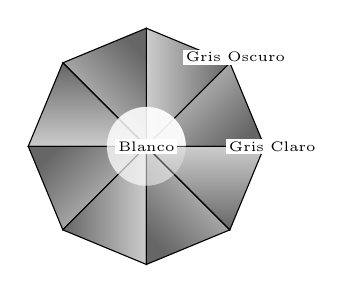
\begin{tikzpicture}
        \coordinate (O) at (0,0);
        % Definición de colores aproximados
        \definecolor{grisclaro}{gray}{0.8}
        \definecolor{grisoscuro}{gray}{0.4}
        
        % Dibujamos cada triángulo interpolando colores (simulado con shade)
        % Nota: TikZ básico no interpola 3 colores por vértice fácilmente en un mesh simple sin librerías extra,
        % aquí usamos un shading radial/axial aproximado para ilustrar el enunciado.
        \foreach \i in {1,...,8} {
            \pgfmathsetmacro{\angleA}{(\i-1)*360/8}
            \pgfmathsetmacro{\angleB}{\i*360/8}
            \shadedraw[shading=axis, bottom color=grisoscuro, top color=grisclaro, shading angle=\angleA+45] 
                (O) -- ({1.5*cos(\angleA)}, {1.5*sin(\angleA)}) -- ({1.5*cos(\angleB)}, {1.5*sin(\angleB)}) -- cycle;
            % Simulamos el centro blanco con un círculo difuso o superposición
            \fill[white, opacity=0.3] (0,0) circle (0.5); 
        }
        % Etiquetas de color para clarificar el requisito
        \node[font=\tiny, fill=white, inner sep=1pt] at (0,0) {Blanco};
        \node[font=\tiny, fill=white, inner sep=1pt] at ({1.6*cos(0)}, {1.6*sin(0)}) {Gris Claro};
        \node[font=\tiny, fill=white, inner sep=1pt] at ({1.6*cos(360/8)}, {1.6*sin(360/8)}) {Gris Oscuro};
    \end{tikzpicture}
    \end{center}
\end{ejercicio}

\begin{solucion} Solución al problema 2.2:
    \lstinputlisting{../code/EjerciciosTeoria/problema_2_2.gd}
    Para ver cuantos vértices tiene la tabla de vértices, hay que tener en cuenta que cada triángulo tiene 3 vértices, y como hay $n$ triángulos, la tabla de vértices debe tener $3n$ vértices. Por lo tanto, la respuesta es $3n$. Siendon $n=8$, la tabla de vértices tiene $24$ vértices.
\end{solucion}

\begin{ejercicio}
    % \textbf{Polígono regular hecho de líneas}

    Repite los dos problemas anteriores (2.1 y 2.2), con los mismos requerimientos, pero ahora usando \textbf{mallas indexadas}, de forma que el número de vértices e índices sea mínimo.

    Responde razonadamente a estas cuestiones:
    \begin{itemize}
        \item ¿Cuántos vértices debe tener ahora la tabla de vértices en cada caso?
        \item ¿Y cuántos índices debe haber?
    \end{itemize}
\end{ejercicio}

\begin{solucion} Solución al problema 2.3:
    \lstinputlisting{../code/EjerciciosTeoria/problema_2_3.gd}
\end{solucion}

\begin{ejercicio}
    \textbf{Aristas del polígono regular}

    Crea un nuevo nodo \texttt{MeshInstance2D} de forma que ahora veamos simplemente las aristas del contorno del polígono regular descrito en los anteriores problemas. En la figura se ve el resultado para $n=16$ y el mismo radio.

    Considera dos casos:
    \begin{enumerate}
        \item Usando una malla \textbf{no indexada}.
        \item Usando una malla \textbf{indexada}.
    \end{enumerate}

    \begin{center}
    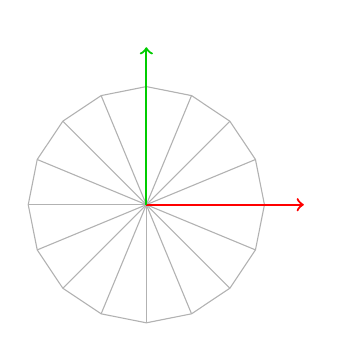
\begin{tikzpicture}
        % Polígono regular de 16 lados (solo contorno)
        \coordinate (center) at (0,0);
        \draw[thin, color=gray!60] (0:1.5)
            \foreach \i in {1,...,15} { -- (\i*360/16:1.5) } -- cycle;
        % Radios
        \foreach \i in {0,...,15} {
            \draw[thin, color=gray!60] (center) -- (\i*360/16:1.5);
        }
        % Ejes de coordenadas
        \draw[->, thick, color=red] (center) -- (0:2) node[right] {};
        \draw[->, thick, color=green!80!black] (center) -- (90:2) node[above] {};
        \end{tikzpicture}
    \end{center}
\end{ejercicio}

\begin{solucion} Solución al problema 2.4:
    \lstinputlisting{../code/EjerciciosTeoria/problema_2_4.gd}
\end{solucion}

\begin{ejercicio}
    \textbf{Generación de malla con segmentos de normales}

    Crea un script global (autoload) con una función que genere un objeto de tipo \texttt{MeshInstance3D} con una malla no indexada que contenga los segmentos representando las normales de una malla dada. La función tendrá la siguiente declaración:

    \begin{verbatim}
func genSegNormales(
    verts: PackedVector3Array, 
    norms: PackedVector3Array,
    lon: float, 
    color: Color 
) -> MeshInstance3D:
    \end{verbatim}

    Donde \texttt{verts} es la tabla de vértices de la malla original, \texttt{norms} la tabla de normales, \texttt{lon} la longitud de los segmentos y \texttt{color} el color de los segmentos. Usa el tipo de primitiva líneas (\texttt{PRIMITIVE\_LINES}), y asegúrate de que a los segmentos no les afecta la iluminación.

    \textbf{Continuación (Uso):}
    Una vez tengas la función disponible, úsala en la función \texttt{\_ready} de alguna malla (por ejemplo, el Donut o los cubos de la práctica), para añadir al objeto un nodo hijo con la malla de segmentos creada por la función.

    Puedes capturar el evento de pulsación de la tecla \textbf{N} del objeto para activar y desactivar la visualización de las normales en ese objeto. Para ello, usa un valor lógico y el atributo de visibilidad de la malla de segmentos.

    \begin{center}
    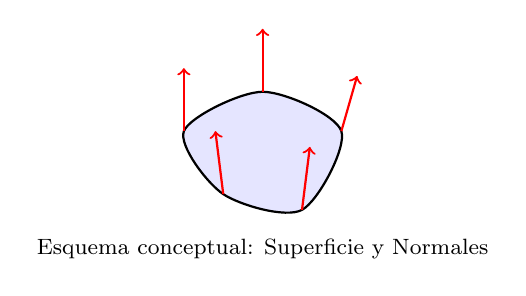
\begin{tikzpicture}
        % Representación esquemática de una superficie con normales
        \draw[thick, fill=blue!10] plot [smooth cycle] coordinates {(0,0) (1,0.5) (2,0) (1.5,-1) (0.5,-0.8)};
        % Normales
        \draw[->, red, thick] (0,0) -- (0, 0.8);
        \draw[->, red, thick] (1,0.5) -- (1, 1.3);
        \draw[->, red, thick] (2,0) -- (2.2, 0.7);
        \draw[->, red, thick] (1.5,-1) -- (1.6, -0.2);
        \draw[->, red, thick] (0.5,-0.8) -- (0.4, 0);
        \node[font=\footnotesize] at (1,-1.5) {Esquema conceptual: Superficie y Normales};
    \end{tikzpicture}
    \end{center}
\end{ejercicio}

\begin{solucion} Solución al problema 2.5:
    Se encuentra en el fichero \texttt{Global.gd} del autoload, cargando anteriormente.
    De todas formas, se añade aquí la función para que se vea más fácilmente:
    \begin{lstlisting}[language=GDScript]
func genSegNormales( verts, norms : PackedVector3Array, lon : float, color : Color ) -> MeshInstance3D:
    var line_verts = PackedVector3Array()
    var line_colors = PackedColorArray()

    for i in range(verts.size()):
        var origen = verts[i]
        var destino = origen + norms[i] * lon

        line_verts.push_back(origen)
        line_verts.push_back(destino)

        line_colors.push_back(color)
        line_colors.push_back(color)

    var arrays = []
    arrays.resize(Mesh.ARRAY_MAX)
    arrays[Mesh.ARRAY_VERTEX] = line_verts
    arrays[Mesh.ARRAY_COLOR] = line_colors

    var arr_mesh = ArrayMesh.new()
    arr_mesh.add_surface_from_arrays(Mesh.PRIMITIVE_LINES, arrays)

    var material = StandardMaterial3D.new()
    material.shading_mode = BaseMaterial3D.SHADING_MODE_UNSHADED
    material.vertex_color_use_as_albedo = true

    var mi = MeshInstance3D.new()
    mi.mesh = arr_mesh
    mi.material_override = material

	return mi
    \end{lstlisting}
\end{solucion}



\section{Sesión 3}

% -------------
% Ejercicios s03
% -------------

% Problema 3.1
\begin{ejercicio}
%\textbf{Problema 3.1: Demostración del cálculo del Producto Escalar}

Demuestra que efectivamente el producto escalar de dos vectores se puede
calcular (usando sus coordenadas en cualquier marco cartesiano) como la
suma del producto componente a componente. Usa las propiedades que
definen dicho producto escalar.
\end{ejercicio}

\begin{solucion}

\textbf{Hipótesis y Datos de Partida:}
\begin{enumerate}
    \item Definimos dos vectores $\vec{u}$ y $\vec{v}$ en un espacio vectorial $V$.
    \item Trabajamos en un \textbf{marco cartesiano}, lo que implica una base ortonormal $\{\hat{e}_i\}$.
    \item Las propiedades de esta base especial son:
    \begin{itemize}
        \item $\hat{e}_i \cdot \hat{e}_i = 1$ (son unitarios).
        \item $\hat{e}_i \cdot \hat{e}_j = 0$ si $i \neq j$ (son perpendiculares).
    \end{itemize}
    \item Expresamos los vectores mediante sus coordenadas en esta base:
    \begin{align*}
        \vec{u} &= \sum_{i=1}^n a_i \hat{e}_i \\
        \vec{v} &= \sum_{j=1}^n b_j \hat{e}_j
    \end{align*}
\end{enumerate}

\textbf{Demostración Paso a Paso:}
\begin{enumerate}
    \item \textbf{Planteamiento del producto:}
    \[
        \vec{u} \cdot \vec{v} = \left( \sum_{i=1}^n a_i \hat{e}_i \right) \cdot \left( \sum_{j=1}^n b_j \hat{e}_j \right)
    \]
    \item \textbf{Aplicación de la Propiedad Distributiva:}
    \[
        = \sum_{i=1}^n \sum_{j=1}^n a_i b_j (\hat{e}_i \cdot \hat{e}_j)
    \]
    \item \textbf{Aplicación de la Propiedad Asociativa (Escalares):}
    Los coeficientes $a_i$ y $b_j$ son reales, así que pueden factorizarse fuera del producto escalar.
    \item \textbf{Aplicación de las Propiedades de la Base Ortonormal:}
    \begin{itemize}
        \item Cuando $i \neq j$, el término es $0$.
        \item Cuando $i = j$, el término es $1$.
    \end{itemize}
    Así, sólo sobreviven los términos con $i = j$:
    \[
        \vec{u} \cdot \vec{v} = \sum_{i=1}^n a_i b_i
    \]
\end{enumerate}

\textbf{Conclusión:} Queda demostrado que, en un marco cartesiano, el producto escalar es la suma de los productos de las componentes homólogas.
\end{solucion}

% Problema 3.2
\begin{ejercicio}
%\textbf{Problema 3.2: Demostración del cálculo del Producto Vectorial}

Demuestra que el producto vectorial de dos vectores se puede calcular usando sus coordenadas en cualquier marco cartesiano según se ha indicado.
\end{ejercicio}

\begin{solucion}
\textbf{Hipótesis y Datos de Partida:}
\begin{enumerate}
    \item Trabajamos en 3D con la base especial $\{\hat{x}, \hat{y}, \hat{z}\}$.
    \item Propiedades definitorias del producto vectorial en esta base:
    \begin{itemize}
        \item $\hat{x} \times \hat{y} = \hat{z}$, $\hat{y} \times \hat{z} = \hat{x}$, $\hat{z} \times \hat{x} = \hat{y}$ (ciclo dextrógiro).
        \item Por la propiedad anticonmutativa, el orden inverso invierte el signo: $\hat{y} \times \hat{x} = -\hat{z}$, etc.
        \item El producto de un vector por sí mismo es nulo: $\hat{x} \times \hat{x} = \vec{0}$, etc.
    \end{itemize}
    \item Vectores definidos por coordenadas:
    \begin{align*}
        \vec{u} &= x_0\hat{x} + y_0\hat{y} + z_0\hat{z} \\
        \vec{v} &= x_1\hat{x} + y_1\hat{y} + z_1\hat{z}
    \end{align*}
\end{enumerate}

\textbf{Demostración Paso a Paso:}
\begin{enumerate}
    \item \textbf{Planteamiento:}
    \[
        \vec{u} \times \vec{v} = (x_0\hat{x} + y_0\hat{y} + z_0\hat{z}) \times (x_1\hat{x} + y_1\hat{y} + z_1\hat{z})
    \]
    \item \textbf{Expansión (Distributiva):}
    \begin{align*}
        &= x_0x_1(\hat{x}\times\hat{x}) + x_0y_1(\hat{x}\times\hat{y}) + x_0z_1(\hat{x}\times\hat{z}) \\
        &\quad + y_0x_1(\hat{y}\times\hat{x}) + y_0y_1(\hat{y}\times\hat{y}) + y_0z_1(\hat{y}\times\hat{z}) \\
        &\quad + z_0x_1(\hat{z}\times\hat{x}) + z_0y_1(\hat{z}\times\hat{y}) + z_0z_1(\hat{z}\times\hat{z})
    \end{align*}
    \item \textbf{Simplificación con Propiedades de la Base:}
    \begin{align*}
        &= 0 + x_0y_1\hat{z} + x_0z_1(-\hat{y}) \\
        &\quad + y_0x_1(-\hat{z}) + 0 + y_0z_1\hat{x} \\
        &\quad + z_0x_1\hat{y} + z_0y_1(-\hat{x}) + 0
    \end{align*}
    \item \textbf{Agrupación por componentes:}
    \begin{align*}
        \text{Componente } \hat{x}: &\quad y_0z_1 - z_0y_1 \\
        \text{Componente } \hat{y}: &\quad z_0x_1 - x_0z_1 \\
        \text{Componente } \hat{z}: &\quad x_0y_1 - y_0x_1
    \end{align*}
    \[
        \vec{u} \times \vec{v} = (y_0z_1 - z_0y_1)\hat{x} + (z_0x_1 - x_0z_1)\hat{y} + (x_0y_1 - y_0x_1)\hat{z}
    \]
\end{enumerate}

\textbf{Conclusión:} El vector resultante en coordenadas es:
\[
    \vec{u} \times \vec{v} = \begin{pmatrix}
        y_0z_1 - z_0y_1 \\
        z_0x_1 - x_0z_1 \\
        x_0y_1 - y_0x_1
    \end{pmatrix}
\]
Esto coincide exactamente con la definición matricial dada en el documento.
\end{solucion}

% Problema 3.3
\begin{ejercicio}
%\textbf{Problema 3.3: Demostración de Ortogonalidad}

Demuestra que el producto vectorial de dos vectores es perpendicular a cada
uno de esos dos vectores.
\end{ejercicio}

\begin{solucion}
\textbf{Datos de Partida:}
\begin{enumerate}
    \item Condición de perpendicularidad: Dos vectores son perpendiculares si su producto escalar es $0$.
    \item Usaremos los resultados demostrados en los Problemas 3.1 y 3.2.
\end{enumerate}

\textbf{Demostración (para $\vec{u}$):}

Queremos probar que $\vec{u} \cdot \vec{w} = 0$.

Sea $\vec{w} = \vec{u} \times \vec{v}$. Sus componentes son (del Prob 3.2):
\begin{align*}
    w_x &= y_0z_1 - z_0y_1 \\
    w_y &= z_0x_1 - x_0z_1 \\
    w_z &= x_0y_1 - y_0x_1
\end{align*}

Calculamos el producto escalar $\vec{u} \cdot \vec{w}$ usando la fórmula de componentes (del Prob 3.1):
\[
    \vec{u} \cdot \vec{w} = x_0w_x + y_0w_y + z_0w_z
\]
Sustituyendo los componentes de $\vec{w}$:
\begin{align*}
    &= x_0(y_0z_1 - z_0y_1) + y_0(z_0x_1 - x_0z_1) + z_0(x_0y_1 - y_0x_1) \\
    &= x_0y_0z_1 - x_0z_0y_1 + y_0z_0x_1 - y_0x_0z_1 + z_0x_0y_1 - z_0y_0x_1
\end{align*}

Reordenamos los términos para ver las cancelaciones:
\begin{itemize}
    \item $x_0y_0z_1$ se cancela con $-y_0x_0z_1$ (son idénticos, el orden de factores reales no altera el producto).
    \item $-x_0z_0y_1$ se cancela con $z_0x_0y_1$.
    \item $y_0z_0x_1$ se cancela con $-z_0y_0x_1$.
\end{itemize}

\textbf{Resultado:}
\[
    \vec{u} \cdot \vec{w} = 0
\]

\textit{(Nota: La demostración para $\vec{v}$ es análoga, sustituyendo las coordenadas de $\vec{v}$ en el producto escalar, y también resultará en $0$).}

\textbf{Conclusión:}
Hemos demostrado algebraicamente la propiedad geométrica fundamental mencionada en la página 30: el producto vectorial genera una dirección perpendicular al plano formado por los dos vectores originales.
\end{solucion}

\begin{ejercicio}
Demuestra que el producto escalar de vectores en 2D es invariante por rotación. Es decir, que para cualquier ángulo $\theta$ y vectores $\vec{u}$ y $\vec{v}$ se cumple:
$$ \vec{u} \cdot \vec{v} = R_\theta(\vec{u}) \cdot R_\theta(\vec{v}) $$
Se requiere realizar la demostración utilizando las coordenadas de los vectores en un marco cartesiano arbitrario.
\end{ejercicio}

\begin{solucion}
Para demostrar la invariancia del producto escalar bajo una transformación de rotación en el espacio euclídeo bidimensional ($\mathbb{R}^2$), procederemos algebraicamente definiendo los componentes de los vectores y la matriz de transformación correspondiente.

Sean $\vec{u}$ y $\vec{v}$ dos vectores libres en $\mathbb{R}^2$ definidos por sus componentes en un marco cartesiano:
$$ \vec{u} = \begin{pmatrix} u_x \\ u_y \end{pmatrix}, \quad \vec{v} = \begin{pmatrix} v_x \\ v_y \end{pmatrix} $$

La definición estándar del producto escalar (producto punto) en coordenadas cartesianas viene dada por:
\begin{equation}
\vec{u} \cdot \vec{v} = u_x v_x + u_y v_y
\end{equation}

Sea $R_\theta$ la transformación de rotación por un ángulo $\theta$ alrededor del origen. La matriz asociada a esta transformación en 2D, $M_R$, se define como:
$$ M_R = \begin{pmatrix} \cos\theta & -\sin\theta \\ \sin\theta & \cos\theta \end{pmatrix} $$

Aplicamos la transformación lineal a los vectores $\vec{u}$ y $\vec{v}$ mediante la multiplicación matricial:

1. Para el vector $\vec{u}' = R_\theta(\vec{u})$:
$$ \vec{u}' = \begin{pmatrix} \cos\theta & -\sin\theta \\ \sin\theta & \cos\theta \end{pmatrix} \begin{pmatrix} u_x \\ u_y \end{pmatrix} = \begin{pmatrix} u_x \cos\theta - u_y \sin\theta \\ u_x \sin\theta + u_y \cos\theta \end{pmatrix} $$
Denotamos las componentes transformadas como $u'_x = u_x \cos\theta - u_y \sin\theta$ y $u'_y = u_x \sin\theta + u_y \cos\theta$.

2. Para el vector $\vec{v}' = R_\theta(\vec{v})$:
$$ \vec{v}' = \begin{pmatrix} \cos\theta & -\sin\theta \\ \sin\theta & \cos\theta \end{pmatrix} \begin{pmatrix} v_x \\ v_y \end{pmatrix} = \begin{pmatrix} v_x \cos\theta - v_y \sin\theta \\ v_x \sin\theta + v_y \cos\theta \end{pmatrix} $$
Denotamos las componentes transformadas como $v'_x = v_x \cos\theta - v_y \sin\theta$ y $v'_y = v_x \sin\theta + v_y \cos\theta$.

Procedemos ahora a calcular el producto escalar de los vectores transformados, $R_\theta(\vec{u}) \cdot R_\theta(\vec{v}) = u'_x v'_x + u'_y v'_y$:

\begin{align*}
R_\theta(\vec{u}) \cdot R_\theta(\vec{v}) &= (u_x \cos\theta - u_y \sin\theta)(v_x \cos\theta - v_y \sin\theta) \\
&\quad + (u_x \sin\theta + u_y \cos\theta)(v_x \sin\theta + v_y \cos\theta)
\end{align*}

Expandimos los términos algebraicos:

\begin{align*}
R_\theta(\vec{u}) \cdot R_\theta(\vec{v}) &= (u_x v_x \cos^2\theta - u_x v_y \cos\theta \sin\theta - u_y v_x \sin\theta \cos\theta + u_y v_y \sin^2\theta) \\
&\quad + (u_x v_x \sin^2\theta + u_x v_y \sin\theta \cos\theta + u_y v_x \cos\theta \sin\theta + u_y v_y \cos^2\theta)
\end{align*}

Agrupamos los términos comunes en función de los coeficientes de los vectores originales:

\begin{align*}
R_\theta(\vec{u}) \cdot R_\theta(\vec{v}) &= u_x v_x (\cos^2\theta + \sin^2\theta) \\
&\quad + u_y v_y (\sin^2\theta + \cos^2\theta) \\
&\quad + u_x v_y (-\cos\theta \sin\theta + \sin\theta \cos\theta) \\
&\quad + u_y v_x (-\sin\theta \cos\theta + \cos\theta \sin\theta)
\end{align*}

Aplicamos la identidad trigonométrica fundamental $\cos^2\theta + \sin^2\theta = 1$ y observamos que los términos cruzados se cancelan:

\begin{align*}
R_\theta(\vec{u}) \cdot R_\theta(\vec{v}) &= u_x v_x (1) + u_y v_y (1) + u_x v_y (0) + u_y v_x (0) \\
&= u_x v_x + u_y v_y
\end{align*}

Comparando este resultado con la definición inicial en la Ecuación (1), concluimos que:
$$ R_\theta(\vec{u}) \cdot R_\theta(\vec{v}) = \vec{u} \cdot \vec{v} $$
Q.E.D.
\end{solucion}

\begin{ejercicio}
Demuestra que en 2D las rotaciones no modifican la longitud de un vector (isometría). Es decir, que para cualquier ángulo $\theta$ y vector $\vec{v}$, se cumple:
$$ \| R_\theta(\vec{v}) \| = \| \vec{v} \| $$
\end{ejercicio}

\begin{solucion}
Para demostrar que la rotación es una transformación isométrica que preserva la norma (longitud) de los vectores, utilizaremos la relación fundamental entre la norma euclídea y el producto escalar.

La definición de la norma de un vector $\vec{v}$ en función del producto escalar es:
$$ \| \vec{v} \| = \sqrt{\vec{v} \cdot \vec{v}} $$
Elevando al cuadrado ambos lados, tenemos:
\begin{equation}
\| \vec{v} \|^2 = \vec{v} \cdot \vec{v}
\end{equation}

Consideremos ahora la norma al cuadrado del vector transformado $R_\theta(\vec{v})$:
$$ \| R_\theta(\vec{v}) \|^2 = R_\theta(\vec{v}) \cdot R_\theta(\vec{v}) $$

Basándonos en la propiedad demostrada en el Ejercicio 3.4 (invariancia del producto escalar bajo rotación), sabemos que para cualesquiera vectores $\vec{a}$ y $\vec{b}$, se cumple $\vec{a} \cdot \vec{b} = R_\theta(\vec{a}) \cdot R_\theta(\vec{b})$.

En este caso particular, hacemos $\vec{a} = \vec{v}$ y $\vec{b} = \vec{v}$. Aplicando la propiedad de invariancia:
$$ R_\theta(\vec{v}) \cdot R_\theta(\vec{v}) = \vec{v} \cdot \vec{v} $$

Sustituyendo esto en la expresión de la norma transformada:
$$ \| R_\theta(\vec{v}) \|^2 = \vec{v} \cdot \vec{v} $$

Dado que $\vec{v} \cdot \vec{v} = \| \vec{v} \|^2$ según la Ecuación (2), obtenemos:
$$ \| R_\theta(\vec{v}) \|^2 = \| \vec{v} \|^2 $$

Tomando la raíz cuadrada positiva en ambos lados (dado que la norma es una magnitud no negativa):
$$ \| R_\theta(\vec{v}) \| = \| \vec{v} \| $$

Por lo tanto, queda demostrado que la aplicación de una matriz de rotación $R_\theta$ no altera la longitud del vector, confirmando que las rotaciones son isometrías.
\end{solucion}

\begin{ejercicio}
Demuestra que si rotamos en 2D un vector +90 grados ($\pi/2$) o -90 grados ($-\pi/2$), obtenemos otro vector perpendicular al original. Es decir, si $\|\theta\| = \pi/2$, entonces:
$$ \vec{v} \cdot R_\theta(\vec{v}) = 0 $$
\end{ejercicio}

\begin{solucion}
Para demostrar la perpendicularidad entre un vector original $\vec{v}$ y su versión rotada $\pm 90^\circ$, utilizaremos la definición algebraica del producto escalar y la matriz de rotación específica para estos ángulos.

Sea $\vec{v}$ un vector arbitrario en $\mathbb{R}^2$:
$$ \vec{v} = \begin{pmatrix} v_x \\ v_y \end{pmatrix} $$

La matriz de rotación general $R_\theta$ es:
$$ R_\theta = \begin{pmatrix} \cos\theta & -\sin\theta \\ \sin\theta & \cos\theta \end{pmatrix} $$

Analizaremos los dos casos solicitados: $\theta = \pi/2$ y $\theta = -\pi/2$.

\textbf{Caso 1: Rotación de $+\pi/2$ ($90^\circ$)}
Sustituimos $\theta = \pi/2$ en la matriz de rotación, sabiendo que $\cos(\pi/2) = 0$ y $\sin(\pi/2) = 1$:
$$ R_{\pi/2} = \begin{pmatrix} 0 & -1 \\ 1 & 0 \end{pmatrix} $$

Calculamos el vector transformado $\vec{v}' = R_{\pi/2}(\vec{v})$:
$$ \vec{v}' = \begin{pmatrix} 0 & -1 \\ 1 & 0 \end{pmatrix} \begin{pmatrix} v_x \\ v_y \end{pmatrix} = \begin{pmatrix} -v_y \\ v_x \end{pmatrix} $$

Ahora calculamos el producto escalar entre el vector original y el transformado:
$$ \vec{v} \cdot \vec{v}' = v_x(-v_y) + v_y(v_x) = -v_x v_y + v_x v_y = 0 $$

\textbf{Caso 2: Rotación de $-\pi/2$ ($-90^\circ$)}
Sustituimos $\theta = -\pi/2$ en la matriz, sabiendo que $\cos(-\pi/2) = 0$ y $\sin(-\pi/2) = -1$:
$$ R_{-\pi/2} = \begin{pmatrix} 0 & 1 \\ -1 & 0 \end{pmatrix} $$

Calculamos el vector transformado $\vec{v}'' = R_{-\pi/2}(\vec{v})$:
$$ \vec{v}'' = \begin{pmatrix} 0 & 1 \\ -1 & 0 \end{pmatrix} \begin{pmatrix} v_x \\ v_y \end{pmatrix} = \begin{pmatrix} v_y \\ -v_x \end{pmatrix} $$

Calculamos el producto escalar:
$$ \vec{v} \cdot \vec{v}'' = v_x(v_y) + v_y(-v_x) = v_x v_y - v_x v_y = 0 $$

\textbf{Conclusión:}
En ambos casos, el producto escalar es nulo. Dado que $\vec{a} \cdot \vec{b} = 0 \iff \vec{a} \perp \vec{b}$ (para vectores no nulos), queda demostrado que el vector rotado $\pm 90^\circ$ es perpendicular al original.
\end{solucion}

\begin{ejercicio}
Demuestra que una matriz de rotación en 2D es siempre ortonormal, independientemente del ángulo. Esto implica demostrar que:
1. Sus filas son ortogonales entre sí (perpendiculares).
2. Sus columnas son ortogonales entre sí.
3. Cada fila y cada columna tiene norma (longitud) igual a 1.
\end{ejercicio}

\begin{solucion}
Una matriz $M$ es ortonormal (u ortogonal) si cumple que $M^T M = I$, lo cual equivale a que sus filas y columnas formen una base ortonormal. Analizaremos las propiedades de filas y columnas de la matriz de rotación general.

Sea $R_\theta$ la matriz de rotación:
$$ R_\theta = \begin{pmatrix} \cos\theta & -\sin\theta \\ \sin\theta & \cos\theta \end{pmatrix} $$

Denotamos las filas como vectores $\vec{r}_1, \vec{r}_2$ y las columnas como $\vec{c}_1, \vec{c}_2$:
$$ \vec{r}_1 = (\cos\theta, -\sin\theta), \quad \vec{r}_2 = (\sin\theta, \cos\theta) $$
$$ \vec{c}_1 = \begin{pmatrix} \cos\theta \\ \sin\theta \end{pmatrix}, \quad \vec{c}_2 = \begin{pmatrix} -\sin\theta \\ \cos\theta \end{pmatrix} $$

\textbf{1. Ortogonalidad de las filas:}
Calculamos el producto escalar $\vec{r}_1 \cdot \vec{r}_2$:
$$ \vec{r}_1 \cdot \vec{r}_2 = (\cos\theta)(\sin\theta) + (-\sin\theta)(\cos\theta) = \sin\theta\cos\theta - \sin\theta\cos\theta = 0 $$
Las filas son perpendiculares.

\textbf{2. Normalidad de las filas (Longitud unitaria):}
Calculamos la norma al cuadrado de cada fila usando la identidad $\cos^2\theta + \sin^2\theta = 1$:
$$ \|\vec{r}_1\|^2 = (\cos\theta)^2 + (-\sin\theta)^2 = \cos^2\theta + \sin^2\theta = 1 \implies \|\vec{r}_1\| = 1 $$
$$ \|\vec{r}_2\|^2 = (\sin\theta)^2 + (\cos\theta)^2 = \sin^2\theta + \cos^2\theta = 1 \implies \|\vec{r}_2\| = 1 $$

\textbf{3. Ortogonalidad de las columnas:}
Calculamos el producto escalar $\vec{c}_1 \cdot \vec{c}_2$:
$$ \vec{c}_1 \cdot \vec{c}_2 = (\cos\theta)(-\sin\theta) + (\sin\theta)(\cos\theta) = -\sin\theta\cos\theta + \sin\theta\cos\theta = 0 $$
Las columnas son perpendiculares.

\textbf{4. Normalidad de las columnas:}
$$ \|\vec{c}_1\|^2 = \cos^2\theta + \sin^2\theta = 1 \implies \|\vec{c}_1\| = 1 $$
$$ \|\vec{c}_2\|^2 = (-\sin\theta)^2 + \cos^2\theta = \sin^2\theta + \cos^2\theta = 1 \implies \|\vec{c}_2\| = 1 $$

\textbf{Conclusión:}
Dado que tanto las filas como las columnas son vectores unitarios y ortogonales entre sí para cualquier valor de $\theta$, la matriz de rotación $R_\theta$ es siempre una matriz ortonormal.
\end{solucion}

\begin{ejercicio}
Demuestra que, en 2D, el producto de una matriz de rotación y una de escalado no es conmutativo en general, excepto si el escalado es uniforme.
\end{ejercicio}

\begin{solucion}
Para analizar la conmutatividad entre la rotación y el escalado, definiremos las matrices correspondientes en el espacio bidimensional. Consideraremos las matrices de $2 \times 2$, dado que ambas son transformaciones lineales y no requieren necesariamente coordenadas homogéneas para demostrar esta propiedad (aunque el resultado es idéntico en $3 \times 3$ con la última fila/columna canónica).

Sean las matrices de rotación $R_\theta$ y de escalado $S(s_x, s_y)$:
$$ R_\theta = \begin{pmatrix} \cos\theta & -\sin\theta \\ \sin\theta & \cos\theta \end{pmatrix}, \quad S = \begin{pmatrix} s_x & 0 \\ 0 & s_y \end{pmatrix} $$

Calculamos el producto $R_\theta \cdot S$ (aplicar escalado y luego rotación):
$$ R_\theta \cdot S = \begin{pmatrix} \cos\theta & -\sin\theta \\ \sin\theta & \cos\theta \end{pmatrix} \begin{pmatrix} s_x & 0 \\ 0 & s_y \end{pmatrix} = \begin{pmatrix} s_x \cos\theta & -s_y \sin\theta \\ s_x \sin\theta & s_y \cos\theta \end{pmatrix} $$

Calculamos el producto $S \cdot R_\theta$ (aplicar rotación y luego escalado):
$$ S \cdot R_\theta = \begin{pmatrix} s_x & 0 \\ 0 & s_y \end{pmatrix} \begin{pmatrix} \cos\theta & -\sin\theta \\ \sin\theta & \cos\theta \end{pmatrix} = \begin{pmatrix} s_x \cos\theta & -s_x \sin\theta \\ s_y \sin\theta & s_y \cos\theta \end{pmatrix} $$

Para que las matrices conmuten, es decir, $R_\theta \cdot S = S \cdot R_\theta$, sus componentes deben ser idénticos término a término. Comparamos los términos fuera de la diagonal principal:

\begin{enumerate}
    \item Elemento $(1,2)$: $-s_y \sin\theta = -s_x \sin\theta \implies (s_x - s_y)\sin\theta = 0$
    \item Elemento $(2,1)$: $s_x \sin\theta = s_y \sin\theta \implies (s_x - s_y)\sin\theta = 0$
\end{enumerate}

Para que la igualdad se cumpla para un ángulo de rotación general ($\sin\theta \neq 0$), es condición necesaria y suficiente que:
$$ s_x = s_y $$

\textbf{Conclusión:}
Si $s_x \neq s_y$ (escalado no uniforme), los productos matriciales son distintos, demostrando que la operación no es conmutativa en general.
Si $s_x = s_y = s$ (escalado uniforme), la matriz de escalado se convierte en $sI$ (donde $I$ es la identidad), la cual conmuta con cualquier matriz cuadrada.
\end{solucion}

\begin{ejercicio}
Demuestra que en 2D, el producto de una matriz de rotación y otra de traslación (por un vector no nulo) no es conmutativo.
\end{ejercicio}

\begin{solucion}
Dado que la traslación es una transformación afín y no lineal, es imprescindible utilizar \textbf{coordenadas homogéneas} para representarla como una multiplicación matricial. Trabajaremos con matrices de $3 \times 3$.

Sea $R_\theta$ la matriz de rotación y $T_{\vec{t}}$ la matriz de traslación por un vector $\vec{t} = (t_x, t_y)$:
$$ R_\theta = \begin{pmatrix} \cos\theta & -\sin\theta & 0 \\ \sin\theta & \cos\theta & 0 \\ 0 & 0 & 1 \end{pmatrix}, \quad T_{\vec{t}} = \begin{pmatrix} 1 & 0 & t_x \\ 0 & 1 & t_y \\ 0 & 0 & 1 \end{pmatrix} $$

Calculamos el producto $R_\theta \cdot T_{\vec{t}}$ (primero se traslada, luego se rota):
$$ R_\theta \cdot T_{\vec{t}} = \begin{pmatrix} \cos\theta & -\sin\theta & 0 \\ \sin\theta & \cos\theta & 0 \\ 0 & 0 & 1 \end{pmatrix} \begin{pmatrix} 1 & 0 & t_x \\ 0 & 1 & t_y \\ 0 & 0 & 1 \end{pmatrix} = \begin{pmatrix} \cos\theta & -\sin\theta & t_x \cos\theta - t_y \sin\theta \\ \sin\theta & \cos\theta & t_x \sin\theta + t_y \cos\theta \\ 0 & 0 & 1 \end{pmatrix} $$
Geométricamente, esto rota el punto y también rota el vector de traslación aplicado.

Calculamos el producto $T_{\vec{t}} \cdot R_\theta$ (primero se rota, luego se traslada):
$$ T_{\vec{t}} \cdot R_\theta = \begin{pmatrix} 1 & 0 & t_x \\ 0 & 1 & t_y \\ 0 & 0 & 1 \end{pmatrix} \begin{pmatrix} \cos\theta & -\sin\theta & 0 \\ \sin\theta & \cos\theta & 0 \\ 0 & 0 & 1 \end{pmatrix} = \begin{pmatrix} \cos\theta & -\sin\theta & t_x \\ \sin\theta & \cos\theta & t_y \\ 0 & 0 & 1 \end{pmatrix} $$
Geométricamente, esto rota el punto alrededor del origen y luego aplica la traslación original sin modificar.

\textbf{Comparación:}
Observamos la tercera columna (la componente de traslación resultante) de ambas matrices resultantes:
$$ \begin{pmatrix} t_x \cos\theta - t_y \sin\theta \\ t_x \sin\theta + t_y \cos\theta \\ 1 \end{pmatrix} \neq \begin{pmatrix} t_x \\ t_y \\ 1 \end{pmatrix} $$

Para que fuesen iguales en un caso general ($\theta \neq 0$), se requeriría que $t_x = 0$ y $t_y = 0$. Dado que el enunciado especifica un vector de traslación no nulo, concluimos que las matrices son distintas.

\textbf{Conclusión:}
El orden de las operaciones altera el resultado final: rotar y luego trasladar lleva a una posición diferente que trasladar y luego rotar (donde el desplazamiento también sufre la rotación). Por tanto, no son conmutativas.
\end{solucion}

\begin{ejercicio}
Demuestra que el producto escalar de vectores en 3D es invariante por rotaciones entorno a los ejes cartesianos, y que estas tampoco modifican la longitud de un vector.
\end{ejercicio}

\begin{solucion}
Para demostrar la invariancia del producto escalar en $\mathbb{R}^3$ bajo rotaciones cartesianas, tomaremos sin pérdida de generalidad el caso de una rotación alrededor del eje $Z$ por un ángulo $\theta$. El procedimiento es análogo para los ejes $X$ e $Y$ debido a la simetría cíclica de las coordenadas.

La matriz de rotación $R_{z,\theta}$ se define como:
$$ R_{z,\theta} = \begin{pmatrix} \cos\theta & -\sin\theta & 0 \\ \sin\theta & \cos\theta & 0 \\ 0 & 0 & 1 \end{pmatrix} $$

Sean $\vec{u} = (u_x, u_y, u_z)$ y $\vec{v} = (v_x, v_y, v_z)$ dos vectores arbitrarios. El producto escalar original es:
\begin{equation}
\vec{u} \cdot \vec{v} = u_x v_x + u_y v_y + u_z v_z
\end{equation}

Calculamos los vectores transformados $\vec{u}' = R_{z,\theta}(\vec{u})$ y $\vec{v}' = R_{z,\theta}(\vec{v})$:
$$ \vec{u}' = \begin{pmatrix} u_x \cos\theta - u_y \sin\theta \\ u_x \sin\theta + u_y \cos\theta \\ u_z \end{pmatrix}, \quad \vec{v}' = \begin{pmatrix} v_x \cos\theta - v_y \sin\theta \\ v_x \sin\theta + v_y \cos\theta \\ v_z \end{pmatrix} $$

Ahora calculamos el producto escalar de los vectores transformados:
\begin{align*}
\vec{u}' \cdot \vec{v}' &= (u_x \cos\theta - u_y \sin\theta)(v_x \cos\theta - v_y \sin\theta) \\
&\quad + (u_x \sin\theta + u_y \cos\theta)(v_x \sin\theta + v_y \cos\theta) \\
&\quad + u_z v_z
\end{align*}

Expandiendo los términos correspondientes a las componentes $x$ e $y$ (idéntico al caso 2D):
\begin{align*}
&= (u_x v_x \cos^2\theta - u_x v_y \cos\theta \sin\theta - u_y v_x \sin\theta \cos\theta + u_y v_y \sin^2\theta) \\
&\quad + (u_x v_x \sin^2\theta + u_x v_y \sin\theta \cos\theta + u_y v_x \cos\theta \sin\theta + u_y v_y \cos^2\theta) \\
&\quad + u_z v_z
\end{align*}

Agrupando y simplificando usando $\sin^2\theta + \cos^2\theta = 1$:
\begin{align*}
\vec{u}' \cdot \vec{v}' &= u_x v_x(\cos^2\theta + \sin^2\theta) + u_y v_y(\sin^2\theta + \cos^2\theta) + u_z v_z \\
&= u_x v_x + u_y v_y + u_z v_z \\
&= \vec{u} \cdot \vec{v}
\end{align*}

\textbf{Invariancia de la longitud:}
Utilizando la relación $\| \vec{v} \|^2 = \vec{v} \cdot \vec{v}$ y la propiedad recién demostrada:
$$ \| R_{z,\theta}(\vec{v}) \|^2 = R_{z,\theta}(\vec{v}) \cdot R_{z,\theta}(\vec{v}) = \vec{v} \cdot \vec{v} = \| \vec{v} \|^2 $$
Tomando la raíz cuadrada, concluimos que $\| R_{z,\theta}(\vec{v}) \| = \| \vec{v} \|$.
\end{solucion}

\begin{ejercicio}
Demuestra que el producto vectorial de dos vectores rota igual que lo hacen esos dos vectores. Es decir, para cualesquiera vectores $\vec{u}, \vec{v}$ y un ángulo $\theta$ con eje $\hat{e}$, se cumple:
$$ R_{\theta,\hat{e}}(\vec{u} \times \vec{v}) = R_{\theta,\hat{e}}(\vec{u}) \times R_{\theta,\hat{e}}(\vec{v}) $$
\end{ejercicio}

\begin{solucion}
Para esta demostración, consideraremos la rotación alrededor del eje $Z$ ($R_{z,\theta}$), ya que la lógica es extensible a cualquier eje cartesiano por permutación de índices.

Definimos $\vec{w} = \vec{u} \times \vec{v}$. Sus componentes son:
$$ \vec{w} = \begin{pmatrix} w_x \\ w_y \\ w_z \end{pmatrix} = \begin{pmatrix} u_y v_z - u_z v_y \\ u_z v_x - u_x v_z \\ u_x v_y - u_y v_x \end{pmatrix} $$

\textbf{Parte 1: Rotación del producto vectorial original ($R_{z,\theta}(\vec{w})$)}
Aplicamos la matriz de rotación al vector $\vec{w}$:
$$ R_{z,\theta}(\vec{w}) = \begin{pmatrix} w_x \cos\theta - w_y \sin\theta \\ w_x \sin\theta + w_y \cos\theta \\ w_z \end{pmatrix} $$
Sustituyendo los componentes de $\vec{w}$:
\begin{equation}
R_{z,\theta}(\vec{w})_x = (u_y v_z - u_z v_y)\cos\theta - (u_z v_x - u_x v_z)\sin\theta
\end{equation}
\begin{equation}
R_{z,\theta}(\vec{w})_y = (u_y v_z - u_z v_y)\sin\theta + (u_z v_x - u_x v_z)\cos\theta
\end{equation}
\begin{equation}
R_{z,\theta}(\vec{w})_z = u_x v_y - u_y v_x
\end{equation}

\textbf{Parte 2: Producto vectorial de los vectores rotados ($\vec{u}' \times \vec{v}'$)}
Sean $\vec{u}' = R_{z,\theta}(\vec{u})$ y $\vec{v}' = R_{z,\theta}(\vec{v})$.
Sus componentes son:
$$ \vec{u}' = (u_x c - u_y s, \ u_x s + u_y c, \ u_z) $$
$$ \vec{v}' = (v_x c - v_y s, \ v_x s + v_y c, \ v_z) $$
(donde $c=\cos\theta, s=\sin\theta$).

Calculamos la componente X de $\vec{u}' \times \vec{v}'$:
\begin{align*}
(\vec{u}' \times \vec{v}')_x &= u'_y v'_z - u'_z v'_y \\
&= (u_x s + u_y c)v_z - u_z(v_x s + v_y c) \\
&= u_x v_z s + u_y v_z c - u_z v_x s - u_z v_y c \\
&= c(u_y v_z - u_z v_y) - s(u_z v_x - u_x v_z)
\end{align*}
Este resultado coincide exactamente con la Ecuación (1).

Calculamos la componente Y de $\vec{u}' \times \vec{v}'$:
\begin{align*}
(\vec{u}' \times \vec{v}')_y &= u'_z v'_x - u'_x v'_z \\
&= u_z(v_x c - v_y s) - (u_x c - u_y s)v_z \\
&= u_z v_x c - u_z v_y s - u_x v_z c + u_y v_z s \\
&= s(u_y v_z - u_z v_y) + c(u_z v_x - u_x v_z)
\end{align*}
Este resultado coincide exactamente con la Ecuación (2).

Calculamos la componente Z de $\vec{u}' \times \vec{v}'$:
\begin{align*}
(\vec{u}' \times \vec{v}')_z &= u'_x v'_y - u'_y v'_x \\
&= (u_x c - u_y s)(v_x s + v_y c) - (u_x s + u_y c)(v_x c - v_y s)
\end{align*}
Desarrollando y simplificando:
\begin{align*}
&= (u_x v_x cs + u_x v_y c^2 - u_y v_x s^2 - u_y v_y sc) - (u_x v_x sc - u_x v_y s^2 + u_y v_x c^2 - u_y v_y cs) \\
&= u_x v_y(c^2 + s^2) - u_y v_x(s^2 + c^2) \\
&= u_x v_y - u_y v_x
\end{align*}
Este resultado coincide con la Ecuación (3).

\textbf{Conclusión:}
Dado que todas las componentes coinciden, queda demostrado que:
$$ R_{z,\theta}(\vec{u} \times \vec{v}) = R_{z,\theta}(\vec{u}) \times R_{z,\theta}(\vec{v}) $$
\end{solucion}

\begin{ejercicio}
    % \textbf{Problema 3.12:}

    Crea un script global (autoload) con una función llamada \texttt{gancho} (sin parámetros) que crea y devuelve un objeto de la clase \texttt{Mesh} con una polilínea azul como la de la figura (los ejes se han dibujado por claridad).

    Crea en tu proyecto un nodo 2D de tipo \texttt{MeshInstance2D} y en \texttt{\_ready} asígnale como malla (propiedad \texttt{mesh}) el objeto resultado de llamar a \texttt{gancho()}, ponle un color azul (propiedad \texttt{modulate}) y verifica que el gancho aparece en pantalla al ejecutar el proyecto.

    \begin{center}
    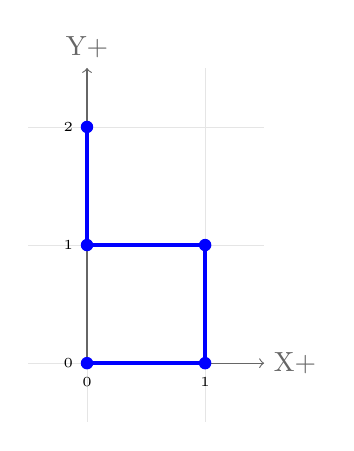
\begin{tikzpicture}[scale=1.5]
        % Rejilla y ejes
        \draw[step=1cm, gray!20, very thin] (-0.5,-0.5) grid (1.5, 2.5);
        \draw[->, black!60] (0,0) -- (1.5,0) node[right] {X+};
        \draw[->, black!60] (0,0) -- (0,2.5) node[above] {Y+};
        \foreach \x in {0,1} \draw (\x,1pt) -- (\x,-1pt) node[anchor=north] {\tiny \x};
        \foreach \y in {0,1,2} \draw (1pt,\y) -- (-1pt,\y) node[anchor=east] {\tiny \y};

        % El gancho
        \draw[blue, ultra thick] (0,0) -- (1,0) -- (1,1) -- (0,1) -- (0,2);
        
        % Puntos destacados (opcional para claridad)
        \fill[blue] (0,0) circle (1.5pt);
        \fill[blue] (1,0) circle (1.5pt);
        \fill[blue] (1,1) circle (1.5pt);
        \fill[blue] (0,1) circle (1.5pt);
        \fill[blue] (0,2) circle (1.5pt);
    \end{tikzpicture}
    \end{center}
\end{ejercicio}

\begin{solucion} Solución al problema 3.12:
    \lstinputlisting{../code/EjerciciosTeoria/problema_3_12.gd}
    Además, añadimos el codigo de gancho que se encuentra en el script global:
    \begin{lstlisting}[language=gdscript]
    func gancho() -> ArrayMesh:
        var vertices = PackedVector2Array([
            Vector2(0,0),
            Vector2(1,0),
            Vector2(1,1),
            Vector2(0,1),
            Vector2(0,2)
        ])

        var arrays = []
        arrays.resize(Mesh.ARRAY_MAX)
        arrays[Mesh.ARRAY_VERTEX] = vertices

        var mesh = ArrayMesh.new()
        mesh.add_surface_from_arrays(Mesh.PRIMITIVE_LINE_STRIP, arrays)
        return mesh
    \end{lstlisting}
\end{solucion}

\begin{ejercicio}
    %\textbf{Problema 3.13:}

    Crea un nodo 2D de tipo \texttt{Node2D} y llámalo \texttt{Gancho\_x4}. En \texttt{\_ready}, añádele cuatro nodos hijos de tipo \texttt{MeshInstance2D}, cada uno de ellos con un malla creada con la función \texttt{gancho} del problema anterior, pero con su \texttt{transform} modificada para que el objeto \texttt{Gancho\_x4} se vea como en la figura (la rejilla y los ejes en rojo se han dibujado por claridad).

    \begin{center}
    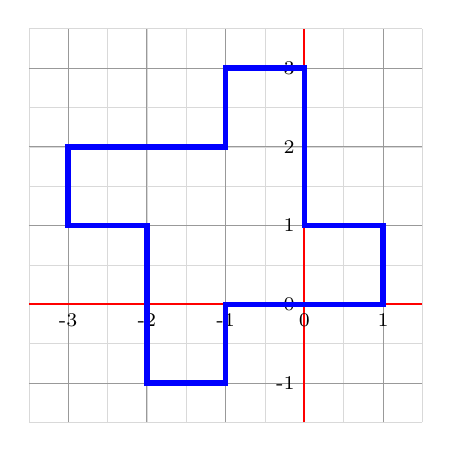
\begin{tikzpicture}[scale=1]
    % 1. Rejilla de fondo (ajustada a los límites de la imagen)
    \draw[step=0.5cm, gray!30, very thin] (-3.5,-1.5) grid (1.5, 3.5);
    \draw[step=1cm, black!40, thin] (-3.5,-1.5) grid (1.5, 3.5);

    % 2. Ejes rojos
    \draw[red, thick] (-3.5,0) -- (1.5,0);
    \draw[red, thick] (0,-1.5) -- (0,3.5);

    % 3. Etiquetas de los ejes
    \foreach \x in {-3,-2,-1,0,1} \node[anchor=north] at (\x,0) {\scriptsize \x};
    \foreach \y in {-1,0,1,2,3} \node[anchor=east] at (0,\y) {\scriptsize \y};

    % 4. El polígono azul continuo
    % He trazado las coordenadas siguiendo tu imagen, empezando en (0,0)
    \draw[blue, line width=2pt] 
        (0,0) -- (1,0) -- (1,1) -- (0,1) --   % Brazo derecho
        (0,3) -- (-1,3) -- (-1,2) --          % Brazo superior (llega a Y=3)
        (-3,2) -- (-3,1) -- (-2,1) --         % Brazo izquierdo (llega a X=-3)
        (-2,-1) -- (-1,-1) -- (-1,0) --       % Brazo inferior (llega a Y=-1)
        cycle;                                % Cierra la figura volviendo a (0,0)

    \end{tikzpicture}
    \end{center}
\end{ejercicio}

\begin{solucion} Solución al problema 3.13:
    \lstinputlisting{../code/EjerciciosTeoria/problema_3_13.gd}
\end{solucion}

\section{Sesión 4}

\begin{ejercicio}
Supongamos que queremos codificar una esfera de radio $1/2$ y centro en el origen de dos formas:

\begin{enumerate}
\item Por enumeración espacial, dividiendo el cubo que engloba a la esfera en celdas, de forma que haya $k$ celdas por lado del cubo, todas ellas son cubos de $1/k$ de ancho. Cada celda ocupa un bit de memoria (si su centro está en la esfera, se guarda un 1, en otro caso un 0).
\item Usando un modelo de fronteras (una malla indexada de triángulos), en el cual se usa una rejilla de triángulos y aristas que siguen los meridianos y paralelos, habiendo en cada meridiano y en cada paralelo un total de $k$ vértices (se guarda únicamente la tabla de vértices y la de triángulos).
\end{enumerate}

Asumiendo que un \texttt{float} y un \texttt{int} ocupan 4 bytes cada uno, contesta a estas cuestiones:

\begin{enumerate}
\item Expresa el tamaño de ambas representaciones en bytes como una función de k.
\item Suponiendo que $k=16$ calcula cuántos KB de memoria ocupa cada estructura.
\item Haz lo mismo asumiendo ahora que $k=1024$ (expresa los resultados en MB).
\item Compara los tamaños de ambas representaciones en ambos casos ($k=16$ y $k=1024$).
\end{enumerate}
\end{ejercicio}

\begin{solucion}
Para resolver este ejercicio, analizaremos detalladamente los requisitos de memoria de cada uno de los modelos propuestos, basándonos en la teoría de representación de modelos geométricos, específicamente la diferencia entre modelos de volúmenes (enumeración espacial) y modelos de fronteras (mallas de polígonos).

\begin{enumerate}
\item \emph{Expresión del tamaño en memoria como función de k.}


Analicemos primero el modelo por \emph{enumeración espacial}.

El espacio que engloba a la esfera de radio $r=1/2$ es un cubo de lado $L = 2r = 1$. Este cubo se discretiza en una rejilla tridimensional de $k$ celdas por lado. Por lo tanto, el número total de celdas (vóxeles) en el volumen es:
\[ N_{celdas} = k \times k \times k = k^3 \]

El enunciado especifica que cada celda ocupa exactamente 1 bit. Para obtener el tamaño en bytes, debemos dividir el número total de bits por 8 (dado que 1 byte = 8 bits).

\[ Mem_{enum}(k) = \frac{k^3}{8} \text{ bytes} \]

Analicemos ahora el modelo de fronteras mediante \emph{malla indexada de triángulos}.

Una malla indexada consta de dos estructuras de datos principales: la tabla de vértices y la tabla de triángulos (índices).

El enunciado indica que la malla se forma siguiendo meridianos y paralelos con $k$ vértices en cada uno. Esto sugiere una topología de rejilla rectangular de dimensiones $k \times k$ mapeada sobre la esfera. En consecuencia, el número de vértices $n_V$ es:
\[ n_V = k^2 \]

Para una malla cerrada y conexa que representa una esfera, topológicamente equivalente a una rejilla envolvente, el número de caras (triángulos) $n_T$ se aproxima al doble del número de vértices (según la característica de Euler para mallas triangulares cerradas donde $n_T \approx 2n_V$). Si consideramos una rejilla de $(k-1) \times (k-1)$ cuadriláteros, y cada cuadrilátero se divide en 2 triángulos, tendríamos $2(k-1)^2$ triángulos. Para valores grandes de $k$, podemos aproximar el número de triángulos como:
\[ n_T \approx 2k^2 \]

Calculamos ahora el uso de memoria para cada tabla:
\begin{enumerate}
    \item \emph{Tabla de vértices:} Cada vértice almacena 3 coordenadas $(x, y, z)$ de tipo \texttt{float}. Si cada \texttt{float} ocupa 4 bytes, el tamaño de un vértice es $3 \times 4 = 12$ bytes.
    \[ Mem_{vert} = 12 \times n_V = 12k^2 \text{ bytes} \]
    
    \item \emph{Tabla de triángulos:} Cada triángulo almacena 3 índices de tipo \texttt{int}. Si cada \texttt{int} ocupa 4 bytes, el tamaño de un triángulo es $3 \times 4 = 12$ bytes.
    \[ Mem_{tri} = 12 \times n_T \approx 12 \times (2k^2) = 24k^2 \text{ bytes} \]
\end{enumerate}

El tamaño total de la malla indexada es la suma de ambas tablas:
\[ Mem_{malla}(k) = 12k^2 + 24k^2 = 36k^2 \text{ bytes} \]

\item \emph{Cálculo de memoria para $k=16$ (en KB).}

Sustituimos $k=16$ en las funciones obtenidas:

Para la \emph{enumeración espacial}:
\[ Mem_{enum}(16) = \frac{16^3}{8} = \frac{4096}{8} = 512 \text{ bytes} \]
Convirtiendo a Kilobytes ($1 \text{ KB} = 1024 \text{ bytes}$):
\[ Mem_{enum}(16) = \frac{512}{1024} = 0.5 \text{ KB} \]

Para la \emph{malla indexada}:
\[ Mem_{malla}(16) = 36 \times 16^2 = 36 \times 256 = 9216 \text{ bytes} \]
Convirtiendo a Kilobytes:
\[ Mem_{malla}(16) = \frac{9216}{1024} = 9 \text{ KB} \]

\item \emph{Cálculo de memoria para $k=1024$ (en MB).}

Sustituimos $k=1024$ en las funciones. Nótese que $1024 = 2^{10}$.

Para la \emph{enumeración espacial}:
\[ Mem_{enum}(1024) = \frac{(2^{10})^3}{2^3} = \frac{2^{30}}{2^3} = 2^{27} \text{ bytes} \]
Sabemos que $1 \text{ MB} = 1024^2 \text{ bytes} = 2^{20} \text{ bytes}$.
\[ Mem_{enum}(1024) = \frac{2^{27}}{2^{20}} = 2^7 = 128 \text{ MB} \]

Para la \emph{malla indexada}:
\[ Mem_{malla}(1024) = 36 \times (1024)^2 = 36 \times 2^{20} \text{ bytes} \]
Convirtiendo a Megabytes:
\[ Mem_{malla}(1024) = 36 \text{ MB} \]

\item \emph{Comparación de tamaños.}

Los resultados obtenidos ilustran la diferencia fundamental en la complejidad espacial entre los modelos volumétricos y los de frontera.

\begin{enumerate}
    \item \emph{Caso $k=16$ (Baja resolución):}
    La enumeración espacial ocupa \emph{menos} memoria ($0.5$ KB) que la malla indexada ($9$ KB). Esto se debe a que, para resoluciones muy bajas, el coste de almacenar coordenadas e índices explícitos (36 bytes por elemento efectivo) supera el coste de almacenar simplemente 1 bit por celda, dado que el volumen total ($k^3$) aún no ha crecido lo suficiente para dominar la expresión.
    
    \item \emph{Caso $k=1024$ (Alta resolución):}
    La enumeración espacial ocupa significativamente \emph{más} memoria ($128$ MB) que la malla indexada ($36$ MB). Aquí se observa la naturaleza cúbica $O(k^3)$ de la enumeración espacial frente a la naturaleza cuadrática $O(k^2)$ del modelo de fronteras. Al aumentar la resolución, el número de celdas interiores (volumen) crece mucho más rápido que el número de vértices necesarios para representar la superficie (área).
\end{enumerate}

\emph{Conclusión:} La enumeración espacial es extremadamente ineficiente en memoria para altas resoluciones, mientras que los modelos de frontera (mallas) son mucho más eficientes para representar objetos sólidos mediante su superficie, especialmente a medida que aumenta la precisión requerida ($k$).



\end{enumerate}
\end{solucion}

\begin{ejercicio}
Considera una malla indexada (tabla de vértices y tabla de caras, esta última con índices de vértices) con una topología de rejilla rectangular. La rejilla está compuesta por $n$ columnas de pares de triángulos y $m$ filas. Esto implica que la estructura tiene $n+1$ columnas de vértices y $m+1$ filas de vértices, con $n, m > 0$.

La figura siguiente ilustra un esquema simplificado de dicha topología (donde los puntos azules representan los vértices y las líneas las aristas que forman los triángulos):

\begin{center}
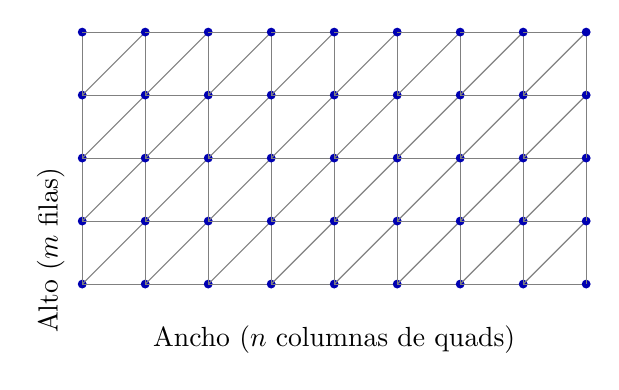
\begin{tikzpicture}[scale=0.8]
% Definición de parámetros para el dibujo
\def\cols{8}
\def\rows{4}
% Dibujar la malla de triángulos
\foreach \y in {0,...,\rows} {
    \foreach \x in {0,...,\cols} {
        % Dibujar vértices
        \fill[blue!70!black] (\x,\y) circle (2pt);
        
        % Dibujar aristas horizontales y verticales (si no estamos en el borde final)
        \ifnum\x<\cols
            \draw[thin, gray] (\x,\y) -- (\x+1,\y);
            % Diagonales y cierres de triángulos
            \ifnum\y<\rows
                \draw[thin, gray] (\x,\y) -- (\x,\y+1);
                \draw[thin, gray] (\x,\y) -- (\x+1,\y+1); % Diagonal
            \fi
        \fi
    }
    % Cerrar el borde derecho vertical
    \ifnum\y<\rows
        \draw[thin, gray] (\cols,\y) -- (\cols,\y+1);
    \fi
}

% Etiquetas
\node[anchor=north] at (\cols/2, -0.5) {Ancho ($n$ columnas de quads)};
\node[anchor=east, rotate=90] at (-0.5, \rows/2) {Alto ($m$ filas)};
\end{tikzpicture}
\end{center}

En relación a este tipo de mallas, responde a las siguientes cuestiones:
\begin{enumerate}[label=(\alph*)]
\item Supongamos que un \texttt{float} ocupa 4 bytes y un \texttt{int} ocupa también 4 bytes. ¿Qué tamaño en memoria ocupa la malla completa en bytes? Ten en cuenta únicamente el tamaño de la tabla de vértices y la tabla de triángulos. Expresa el tamaño como una función de $m$ y $n$.
\item Calcula el tamaño exacto en KiloBytes (KB) suponiendo que $m = n = 128$.
\item Supongamos que $m$ y $n$ son ambos grandes (es decir, asumimos que términos como $1/n$ y $1/m$ son despreciables frente a 1). Deduce qué relación aproximada existe entre el número de caras ($n_C$) y el número de vértices ($n_V$) en este tipo de mallas.
\end{enumerate}
\end{ejercicio}

\begin{solucion}
Para resolver este problema, analizaremos por separado el consumo de memoria de la geometría (tabla de vértices) y de la topología (tabla de triángulos).

\begin{enumerate}[label=(\alph*)]
\item \textbf{Cálculo de la función de memoria $Mem(m, n)$ en bytes}

Primero determinamos la cantidad de elementos:
\begin{itemize}
    \item \textbf{Número de vértices ($n_V$):} 
    La rejilla tiene $m$ filas de celdas y $n$ columnas de celdas. Los vértices se sitúan en las intersecciones.
    \[ \text{Filas de vértices} = m + 1 \]
    \[ \text{Columnas de vértices} = n + 1 \]
    \[ n_V = (m+1)(n+1) \]
    
    \item \textbf{Número de caras/triángulos ($n_C$):}
    Cada celda de la rejilla (formada por la intersección de una fila y una columna) es un cuadrilátero dividido en 2 triángulos.
    \[ \text{Número de celdas} = m \times n \]
    \[ n_C = 2 \times (m \times n) = 2mn \]
\end{itemize}

Ahora calculamos el uso de memoria sabiendo que 1 \texttt{float} = 4 bytes y 1 \texttt{int} = 4 bytes:

\begin{itemize}
    \item \textbf{Memoria de la Tabla de Vértices ($M_V$):}
    Cada vértice almacena 3 coordenadas ($x, y, z$) de tipo \texttt{float}.
    \[ M_V = n_V \times 3 \times 4 \text{ bytes} = 12(m+1)(n+1) \text{ bytes} \]
    
    \item \textbf{Memoria de la Tabla de Triángulos ($M_T$):}
    Cada triángulo almacena 3 índices de vértices ($i, j, k$) de tipo \texttt{int}.
    \[ M_T = n_C \times 3 \times 4 \text{ bytes} = 12 \times (2mn) \text{ bytes} = 24mn \text{ bytes} \]
\end{itemize}

\textbf{Memoria Total ($Mem$):}
\[ Mem(m, n) = M_V + M_T \]
\[ Mem(m, n) = 12(mn + m + n + 1) + 24mn \]
Agrupando términos semejantes:
\[ Mem(m, n) = 12mn + 12m + 12n + 12 + 24mn \]
\[ \boxed{Mem(m, n) = 36mn + 12m + 12n + 12 \text{ bytes}} \]

\item \textbf{Cálculo para $m = n = 128$}

Sustituimos $m$ y $n$ por 128 en la fórmula obtenida:
\[ Mem(128, 128) = 36(128 \times 128) + 12(128) + 12(128) + 12 \]
\[ Mem(128, 128) = 36(16384) + 1536 + 1536 + 12 \]
\[ Mem(128, 128) = 589824 + 3084 \]
\[ Mem(128, 128) = 592908 \text{ bytes} \]

Para convertir a KiloBytes (KB), dividimos por 1024:
\[ \text{Memoria en KB} = \frac{592908}{1024} \approx 579.01 \text{ KB} \]

\textbf{Resultado:} Aproximadamente \textbf{579 KB}.

\item \textbf{Relación asintótica entre $n_C$ y $n_V$}

Partimos de las expresiones deducidas en el apartado (a):
\[ n_V = (m+1)(n+1) = mn + m + n + 1 \]
\[ n_C = 2mn \]

Si asumimos que $m$ y $n$ son grandes, los términos lineales ($m, n$) y el término constante ($1$) son despreciables frente al término cuadrático ($mn$). Matemáticamente:
\[ \lim_{m,n \to \infty} \frac{n_V}{mn} = \lim_{m,n \to \infty} \frac{mn + m + n + 1}{mn} = 1 \]
Por tanto, para valores grandes, podemos aproximar:
\[ n_V \approx mn \]

\textit{Nota: se divide por el término de mayor grado porque de esta manera, en matemáticas, vemos como se comporta en el infinito, otra opción es el mismo límite de nc/nv.}

Calculamos la relación (ratio) entre el número de caras y el número de vértices:
\[ \frac{n_C}{n_V} \approx \frac{2mn}{mn} = 2 \]

\textbf{Conclusión:} En mallas cerradas o mallas de rejilla densas (donde los efectos de borde son insignificantes), \textbf{el número de caras (triángulos) es aproximadamente el doble que el número de vértices}:
\[ n_C \approx 2 n_V \]
\end{enumerate}
\end{solucion}

\begin{ejercicio}

Imagina de nuevo una malla con topología de rejilla, en la cual hay $n$ columnas de pares de triángulos y $m$ filas. Supongamos que usamos una representación como \textbf{tiras de triángulos} (Triangle Strips), de forma que cada fila de triángulos (con $2n$ triángulos) se almacena en una tira independiente, habiendo un total de $m$ tiras.

La estructura de datos consta de una tabla de punteros a tiras (que tiene un entero para el número de tiras y $m$ punteros, donde cada puntero ocupa 8 bytes) y los arrays de coordenadas de las tiras. Asume que las coordenadas son de tipo \texttt{float} (4 bytes) y que no se usan índices (las coordenadas se almacenan explícitamente en el orden de la tira).

Responde a las siguientes cuestiones:
\begin{enumerate}[label=(\alph*)]
    \item Indica qué cantidad de memoria ocupa esta representación en dos casos:
    \begin{enumerate}[label=(\arabic*)]
        \item Como función de $n$ y $m$, en bytes.
        \item Suponiendo $m=n=128$, en KB.
    \end{enumerate}
    \item Para $m$ y $n$ grandes (asumiendo que los términos lineales son despreciables frente a los cuadráticos), describe qué relación hay entre el tamaño en memoria de la malla indexada (Problema 4.2) y el tamaño de la malla almacenada como tiras de triángulos.
    \item Si suponemos que la transformación de cada vértice se hace en un tiempo constante igual a la unidad, describe qué relación hay entre los tiempos de procesamiento de vértices para esta malla cuando se representa como una malla indexada y como tiras de triángulos.
\end{enumerate}
\end{ejercicio}

\begin{solucion}
% \section*{Análisis de la Estructura de Tiras}

Para resolver este ejercicio, primero debemos determinar cuántos vértices se almacenan explícitamente en una tira de triángulos que representa una fila de la rejilla.

\begin{itemize}
    \item Una tira de triángulos que contiene $k$ triángulos requiere $k+2$ vértices. Básicamente, sabemos que cada nuevo triángulo en la tira comparte dos vértices con el triángulo anterior, si para 2 triangulos necesitamos 4 vértices, por inducción (3 vértices $\times$ (k-1) restantes $\times$ 1 vértice que añadimos) se llega a la fórmula $k + 2$.
    \item En la rejilla descrita, cada fila contiene $n$ celdas cuadradas (pares de triángulos). Por lo tanto, el número de triángulos por fila (por tira) es $k = 2n$.
    \item El número de vértices almacenados por cada tira es:
    $$
    V_{tira} = (2n) + 2 = 2n + 2
    $$
    \item Cada vértice consta de 3 coordenadas ($x, y, z$) de tipo \texttt{float} (4 bytes cada uno). El tamaño de un vértice es:
    $$
    B_{vertice} = 3 \times 4 \text{ bytes} = 12 \text{ bytes}
    $$
\end{itemize}

\begin{center}
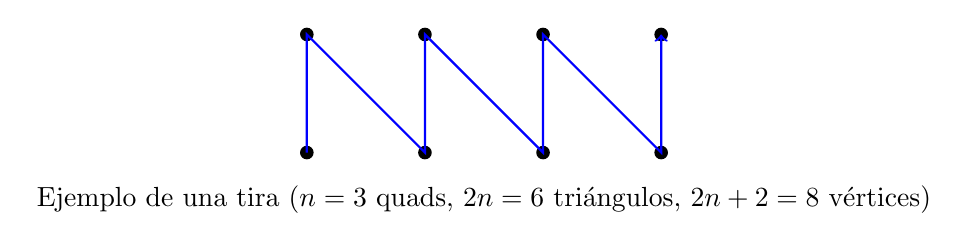
\begin{tikzpicture}[scale=1.5]
% Draw grid points and strip path
\foreach \x in {0,1,2,3} {\foreach \y in {0,1} {\filldraw (\x,\y) circle (1.5pt);}}
% Draw strip lines (zig-zag)
\draw[blue, thick, ->] (0,0) -- (0,1) -- (1,0) -- (1,1) -- (2,0) -- (2,1) -- (3,0) -- (3,1);
\node[below] at (1.5, -0.2) {Ejemplo de una tira ($n=3$ quads, $2n=6$ triángulos, $2n+2=8$ vértices)};
\end{tikzpicture}
\end{center}

\underline{(a) Cálculo de Memoria}

\textbf{(1) Función de $n$ y $m$ en bytes}

El tamaño total $M_{total}$ se compone del tamaño de los datos de las tiras y la sobrecarga de la estructura de punteros.

\begin{enumerate}
    \item \textbf{Memoria de los vértices:} Hay $m$ tiras.
    $$
    M_{geom} = m \times (2n + 2) \text{ vértices} \times 12 \text{ bytes/vértice}
    $$
    $$
    M_{geom} = 12m(2n + 2) = 24nm + 24m \text{ bytes}
    $$
    \item \textbf{Memoria de la tabla de punteros:} Contiene 1 entero (4 bytes) y $m$ punteros (8 bytes c/u\footnote{cada uno}).
    $$
    M_{estructura} = 4 + 8m \text{ bytes}
    $$
    \item \textbf{Memoria Total:}
    $$
    M_{total}(n, m) = (24nm + 24m) + (8m + 4)
    $$
    $$
    \boxed{M_{total}(n, m) = 24nm + 32m + 4 \text{ bytes}}
    $$
\end{enumerate}

\textbf{(2) Cálculo para $m=n=128$}

Sustituimos los valores en la fórmula obtenida:
$$
M_{total}(128, 128) = 24(128 \times 128) + 32(128) + 4
$$
$$
M_{total} = 24(16384) + 4096 + 4
$$
$$
M_{total} = 393216 + 4096 + 4 = 397316 \text{ bytes}
$$

Para convertir a Kilobytes (asumiendo $1 \text{ KB} = 1024 \text{ bytes}$):
$$
M_{KB} = \frac{397316}{1024} \approx \boxed{388.00 \text{ KB}}
$$



\underline{(b) Relación de tamaño con Malla Indexada}

Para $n, m$ grandes, solo consideramos los términos de mayor orden ($nm$).

\textbf{1. Tamaño Malla Indexada (del Problema 4.2):}
\begin{itemize}
    \item Vértices únicos: $\approx nm$. Tamaño: $nm \times 12$ bytes.
    \item Triángulos: $\approx 2nm$. Índices: $2nm \times 3 \text{ índices} \times 4 \text{ bytes} = 24nm$ bytes. El cálculo de los índices ha sido número de triángulos por 3 índices por triángulo por 4 bytes por índice.
    \item Total Indexada: $12nm + 24nm = \mathbf{36nm}$ bytes.
\end{itemize}

\textbf{2. Tamaño Tiras de Triángulos (obtenido en a):}
\begin{itemize}
    \item Total Tiras: $\mathbf{24nm}$ bytes.
\end{itemize}

\textbf{Comparación:}

Calculamos la relación (ratio) entre ambas representaciones:
$$
\frac{\text{Memoria Tiras}}{\text{Memoria Indexada}} \approx \frac{24nm}{36nm} = \frac{2}{3}
$$

\textbf{Conclusión:}

La representación mediante tiras de triángulos ocupa aproximadamente \textbf{el 66.6\% (dos tercios)} de la memoria que ocupa la malla indexada para esta topología de rejilla. Esto se debe a que, aunque las tiras duplican los vértices compartidos entre filas adyacentes, evitan el coste de almacenar 3 enteros por cada triángulo, que es más costoso que almacenar coordenadas repetidas en este escenario específico.



\underline{(c) Comparación de tiempos de procesamiento}

El tiempo de procesamiento de vértices ($T_{proc}$) en la GPU depende del número de veces que se debe ejecutar el \textit{Vertex Shader}.

\textbf{1. Malla Indexada:}

Gracias al \textit{Post-Transform Cache} de la GPU, los vértices indexados suelen procesarse una sola vez por cada vértice único (idealmente).
$$
V_{unicos} \approx nm \implies T_{index} \propto nm
$$

\textbf{2. Tiras de Triángulos (No Indexadas):}

En la implementación descrita (arrays de arrays), los vértices se envían explícitamente por cada tira. Los vértices que se encuentran en la frontera entre la fila $i$ y la fila $i+1$ están duplicados en memoria (aparecen en la tira $i$ y en la tira $i+1$). La GPU no sabe que son el mismo vértice geométrico y debe procesarlos dos veces.
$$
V_{tiras} = m(2n+2) \approx 2nm \implies T_{tiras} \propto 2nm
$$

\textbf{Conclusión:}
$$
\frac{T_{tiras}}{T_{index}} \approx \frac{2nm}{nm} = 2
$$

El tiempo de procesamiento usando tiras de triángulos independientes (no indexadas) es aproximadamente \textbf{el doble} que usando una malla indexada. Aunque las tiras ahorran memoria de almacenamiento en disco/RAM en este caso, son menos eficientes computacionalmente porque obligan a la GPU a transformar los mismos vértices frontera múltiples veces.
\end{solucion}

\begin{ejercicio}

Supongamos una malla cerrada, simplemente conexa (topológicamente equivalente a una esfera), cuyas caras son triángulos y cuyas aristas son todas adyacentes a exactamente dos caras (la malla es un poliedro simplemente conexo de caras triangulares).

Considera el número de vértices $n_V$, el número de aristas $n_A$ y el número de caras $n_C$ en este tipo de mallas.

Demuestra que cualquiera de esos números determina a los otros dos, en concreto, demuestra que se cumplen estas dos igualdades:
$$n_A = 3(n_V - 2)$$
$$n_C = 2(n_V - 2)$$
\end{ejercicio}

\begin{solucion}
Para demostrar las igualdades propuestas, utilizaremos dos propiedades fundamentales de la topología de superficies cerradas y de las mallas triangulares. Procederemos paso a paso estableciendo un sistema de ecuaciones.

\begin{enumerate}
\item \textbf{Aplicación de la Fórmula de Euler-Poincaré:}

Dado que el enunciado especifica que la malla es cerrada y topológicamente equivalente a una esfera (género $g=0$), se cumple la característica de Euler para poliedros convexos:
\begin{equation}
n_V - n_A + n_C = 2 \label{eq:euler}
\end{equation}
Donde:
\begin{itemize}
\item $n_V$: Número de vértices.
\item $n_A$: Número de aristas.
\item $n_C$: Número de caras.
\end{itemize}

\item \textbf{Relación de adyacencia Caras-Aristas:}

En una malla compuesta exclusivamente por triángulos, cada cara tiene exactamente 3 aristas. Además, al ser una variedad cerrada (manifold), cada arista es compartida exactamente por 2 caras.

Podemos contar el número total de ''lados'' de los triángulos de dos formas:
\begin{itemize}
    \item Multiplicando el número de caras por 3: $3 \cdot n_C$.
    \item Multiplicando el número de aristas por 2 (ya que cada arista cuenta para dos caras): $2 \cdot n_A$.
\end{itemize}
Igualando ambas cantidades obtenemos la segunda ecuación fundamental:
\begin{equation}
    3n_C = 2n_A \implies n_C = \frac{2}{3}n_A \quad \text{o bien} \quad n_A = \frac{3}{2}n_C \label{eq:adyacencia}
\end{equation}

\item \textbf{Demostración de $n_C = 2(n_V - 2)$:}

Sustituimos $n_A$ en la Ecuación (\ref{eq:euler}) utilizando la relación obtenida en (\ref{eq:adyacencia}) ($n_A = \frac{3}{2}n_C$):
$$n_V - \left(\frac{3}{2}n_C\right) + n_C = 2$$
Multiplicamos toda la ecuación por 2 para eliminar la fracción:
$$2n_V - 3n_C + 2n_C = 4$$
Simplificamos los términos de $n_C$:
$$2n_V - n_C = 4$$
Despejamos $n_C$:
$$n_C = 2n_V - 4$$
Factorizamos el 2:
$$\boxed{n_C = 2(n_V - 2)}$$
\textit{Q.E.D. (Queda demostrado que el número de caras es aproximadamente el doble que el de vértices).}

\item \textbf{Demostración de $n_A = 3(n_V - 2)$:}

Partimos de nuevo de la Ecuación (\ref{eq:euler}), pero esta vez sustituimos $n_C$ despejándolo de (\ref{eq:adyacencia}) como $n_C = \frac{2}{3}n_A$:
$$n_V - n_A + \left(\frac{2}{3}n_A\right) = 2$$
Multiplicamos toda la ecuación por 3 para eliminar la fracción:
$$3n_V - 3n_A + 2n_A = 6$$
Simplificamos los términos de $n_A$:
$$3n_V - n_A = 6$$
Despejamos $n_A$:
$$n_A = 3n_V - 6$$
Factorizamos el 3:
$$\boxed{n_A = 3(n_V - 2)}$$
\end{enumerate}

\begin{center}
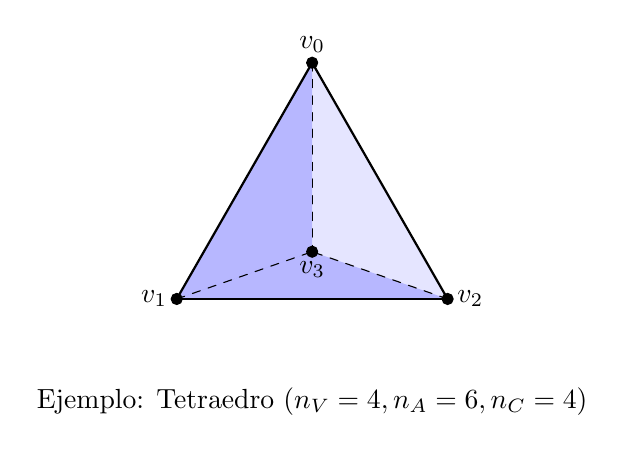
\begin{tikzpicture}[scale=2, line join=round, line cap=round]
% Visualización de un Tetraedro (Malla triangular cerrada más simple)
% nV=4, nC=4, nA=6.
% Comprobación: nC = 2(4-2) = 4. nA = 3(4-2) = 6.
\coordinate (A) at (0,1);
\coordinate (B) at (-0.86,-0.5);
\coordinate (C) at (0.86,-0.5);
\coordinate (D) at (0, -0.2); % Vértice ''oculto/central'' proyectado

% Caras
\fill[opacity=0.1, blue] (A) -- (B) -- (C) -- cycle;
\fill[opacity=0.2, blue] (A) -- (B) -- (D) -- cycle;
\fill[opacity=0.2, blue] (B) -- (C) -- (D) -- cycle;

% Aristas
\draw[thick] (A) -- (B);
\draw[thick] (B) -- (C);
\draw[thick] (C) -- (A);
\draw[dashed] (A) -- (D);
\draw[dashed] (B) -- (D);
\draw[dashed] (C) -- (D);

% Etiquetas
\foreach \p in {A,B,C,D} \filldraw [black] (\p) circle (1pt);
\node[above] at (A) {$v_0$};
\node[left] at (B) {$v_1$};
\node[right] at (C) {$v_2$};
\node[below] at (D) {$v_3$};

\node[below=1cm] at (0,-0.5) {Ejemplo: Tetraedro ($n_V=4, n_A=6, n_C=4$)};
\end{tikzpicture}
\end{center}
\end{solucion}


\begin{ejercicio}

En una malla indexada, queremos añadir a la estructura de datos una tabla de aristas. Será un vector \texttt{ari}, que en cada entrada tendrá una tupla de tipo \texttt{Vector2i} (contiene dos \texttt{int}) con los índices en la tabla de vértices de los dos vértices en los extremos de la arista. El orden en el que aparecen los vértices en una arista es indiferente, pero cada arista debe aparecer una sola vez.

Escribe el código de una función GDScript para crear y calcular la tabla de aristas a partir de la tabla de triángulos. Intenta encontrar una solución con la mínima complejidad en tiempo y memoria posible. Suponer que el número de vértices adyacentes a uno cualquiera de ellos es como mucho un valor constante $k > 0$, valor que no depende del número total de vértices, que llamamos $n$.

Considerar dos casos:
\begin{enumerate}[label=(\alph*)]
\item Los triángulos se dan con orientación no coherente: esto quiere decir que si un triángulo está formado por los vértices $i, j, k$, estos tres índices pueden aparecer en cualquier orden en la correspondiente entrada de la tabla de triángulos. Además, no sabemos si la malla es cerrada o no.
\item Los triángulos se dan con orientación coherente: esto quiere decir que si dos triángulos comparten una arista entre los vértices $i$ y $j$, entonces en uno de los triángulos la arista aparece como $(i, j)$ y en el otro aparece como $(j, i)$. Además, asumimos que la malla es cerrada, es decir, que cada arista es compartida por exactamente dos triángulos.
\end{enumerate}
\end{ejercicio}

\begin{solucion}
Para resolver este problema, debemos iterar sobre la tabla de triángulos y extraer las aristas potenciales. La diferencia fundamental entre los dos casos radica en cómo garantizamos la unicidad de las aristas (evitar duplicados) de manera eficiente.

\underline{\textbf{Caso (a): Orientación no coherente y malla general}}

En este escenario, no podemos predecir el orden de los índices ni cuántas veces aparece una arista (podría ser 1 si es frontera, o 2 si es interna, o más si la malla no es ''manifold'').

\textbf{Estrategia:}
\begin{enumerate}
\item Recorremos cada triángulo y extraemos sus 3 aristas: $(v_0, v_1)$, $(v_1, v_2)$ y $(v_2, v_0)$.
\item Para identificar una arista de forma única sin importar el orden (es decir, que la arista $i-j$ sea igual a $j-i$), ordenamos los índices de cada par: guardamos siempre $(\min(i,j), \max(i,j))$.
\item Usamos una estructura de datos tipo \textit{Set} (Conjunto) o un Diccionario para almacenar las aristas encontradas. Esto elimina duplicados automáticamente con una complejidad promedio de $O(1)$ por inserción.
\end{enumerate}

\textbf{Código GDScript:}
\begin{lstlisting}
func calcular_aristas_caso_a(triangulos: Array[Vector3i]) -> Array[Vector2i]:
    var aristas_unicas = {} # Usamos un diccionario como Set
    for t in triangulos:
        # Extraemos los 3 pares de vértices
        var pares = [
            Vector2i(t[0], t[1]),
            Vector2i(t[1], t[2]),
            Vector2i(t[2], t[0])
        ]
        for par in pares:
            # Normalizamos la arista: (menor, mayor)
            var a = par.x
            var b = par.y
            var key: Vector2i
            if a < b:
                key = Vector2i(a, b)
            else:
                key = Vector2i(b, a)
            # Insertamos en el diccionario (la clave evita duplicados)
            aristas_unicas[key] = true
    # Convertimos las claves del diccionario a un Array
    var ari: Array[Vector2i] = []
    for key in aristas_unicas.keys():
        ari.append(key)
    return ari
\end{lstlisting}

\textbf{Complejidad:}
\begin{itemize}
\item Tiempo: $O(N_t)$, donde $N_t$ es el número de triángulos (asumiendo inserción en hash map constante).
\item Memoria: $O(N_a)$, donde $N_a$ es el número de aristas únicas, necesario para el diccionario auxiliar.
\end{itemize}

\underline{\textbf{Caso (b): Orientación coherente y malla cerrada}}

En este escenario, tenemos una propiedad topológica fuerte: cada arista interna es compartida por exactamente dos triángulos. Debido a la orientación coherente, si la arista conecta los vértices A y B:
\begin{itemize}
\item En el Triángulo 1 aparecerá como secuencia $\dots \rightarrow A \rightarrow B \rightarrow \dots$
\item En el Triángulo 2 aparecerá como secuencia $\dots \rightarrow B \rightarrow A \rightarrow \dots$
\end{itemize}

\textbf{Estrategia:}
Para evitar duplicados sin usar memoria extra (diccionarios), podemos aplicar una regla de selección simple: \textbf{Solo añadimos la arista si el índice de origen es menor que el índice de destino ($i < j$)}.
\begin{itemize}
\item Cuando procesemos el par $(i, j)$ donde $i < j$, lo guardamos.
\item Cuando procesemos el par $(j, i)$ (que existirá obligatoriamente en el triángulo vecino), como $j > i$, lo ignoramos.
\end{itemize}
Esto garantiza que cada arista se añade exactamente una vez.

\textbf{Código GDScript:}
\begin{lstlisting}
func calcular_aristas_caso_b(triangulos: Array[Vector3i]) -> Array[Vector2i]:
    var ari: Array[Vector2i] = []
    for t in triangulos:
        # Definimos los 3 pares tal cual aparecen en el orden del triángulo
        # Arista 0-1
        if t[0] < t[1]:
            ari.append(Vector2i(t[0], t[1]))
        # Arista 1-2
        if t[1] < t[2]:
            ari.append(Vector2i(t[1], t[2]))
        # Arista 2-0
        if t[2] < t[0]:
            ari.append(Vector2i(t[2], t[0]))
    return ari
\end{lstlisting}

\textbf{Complejidad:}
\begin{itemize}
\item Tiempo: $O(N_t)$. Es extremadamente rápido porque solo implica comparaciones de enteros.
\item Memoria: $O(1)$ de memoria auxiliar (no necesitamos estructuras intermedias como diccionarios, escribimos directamente en el resultado).
\end{itemize}
\end{solucion}

\begin{ejercicio}

Escribe el pseudo-código de la función para calcular el área total de una malla indexada de triángulos, a partir de la tabla de vértices y de la tabla de triángulos.

Será una función GDScript que acepta ambas tablas:
\begin{itemize}
\item \texttt{vertices}: un array de tipo \texttt{Vector3} que contiene las posiciones espaciales.
\item \texttt{triangulos}: un array de tipo \texttt{Vector3i}, donde cada elemento contiene los tres índices enteros que forman una cara.
\end{itemize}
La función debe devolver el área total como un valor de punto flotante (\texttt{float}).
\end{ejercicio}

\begin{solucion}
Para resolver este problema, debemos basarnos en la geometría vectorial. El área de cualquier polígono complejo en 3D (la malla) es la suma de las áreas de sus primitivas individuales (los triángulos).

\subsubsection*{Fundamento Matemático}
El área de un triángulo en el espacio 3D definido por tres puntos $P_0, P_1, P_2$ se puede calcular utilizando el \textbf{producto vectorial} (o producto cruz).

\begin{enumerate}
\item Definimos dos vectores que representen dos lados del triángulo partiendo de un vértice común, por ejemplo $P_0$:
$$\vec{u} = P_1 - P_0$$
$$\vec{v} = P_2 - P_0$$
\item El producto vectorial $\vec{w} = \vec{u} \times \vec{v}$ genera un vector perpendicular al plano del triángulo.
\item La magnitud (o longitud) de este vector resultante, $||\vec{w}||$, es igual al área del \textbf{paralelogramo} formado por los vectores $\vec{u}$ y $\vec{v}$.
\item Dado que un triángulo es la mitad de un paralelogramo, el área del triángulo es la mitad de dicha magnitud:
$$\text{Área}_{tri} = \frac{1}{2} ||\vec{u} \times \vec{v}||$$
\end{enumerate}

\begin{center}
\begin{tikzpicture}[scale=2]
% Coordenadas
\coordinate (P0) at (0,0);
\coordinate (P1) at (2,0.5);
\coordinate (P2) at (0.5, 1.5);
% Relleno triángulo
\fill[blue!10] (P0) -- (P1) -- (P2) -- cycle;

% Vectores
\draw[->, thick, blue] (P0) -- (P1) node[midway, below right] {$\vec{u} = P_1 - P_0$};
\draw[->, thick, red] (P0) -- (P2) node[midway, left] {$\vec{v} = P_2 - P_0$};

% Vértices
\filldraw (P0) circle (1pt) node[below left] {$P_0$};
\filldraw (P1) circle (1pt) node[right] {$P_1$};
\filldraw (P2) circle (1pt) node[above] {$P_2$};

% Paralelogramo fantasma
\coordinate (P3) at (2.5, 2.0);
\draw[dashed, gray] (P1) -- (P3) -- (P2);

\node at (2.5, 1) {\small $||\vec{u} \times \vec{v}|| = \text{Área Paralelogramo}$};
\end{tikzpicture}
\end{center}

\subsubsection*{Implementación en GDScript}
El algoritmo consiste en iterar sobre la tabla de triángulos, recuperar las coordenadas de los vértices usando los índices, calcular el área de cada triángulo individual y acumularla en una variable total.

\begin{lstlisting}
func calcular_area_malla(vertices: Array[Vector3], triangulos: Array[Vector3i]) -> float:
    var area_total: float = 0.0
    for t in triangulos:
        var p0: Vector3 = vertices[t[0]]
        var p1: Vector3 = vertices[t[1]]
        var p2: Vector3 = vertices[t[2]]
        var u: Vector3 = p1 - p0
        var v: Vector3 = p2 - p0
        var vector_area: Vector3 = u.cross(v)
        var area_triangulo: float = vector_area.length() * 0.5
        area_total += area_triangulo
    return area_total
\end{lstlisting}

\textbf{Análisis de complejidad:} Si $N_t$ es el número de triángulos (longitud del array \texttt{triangulos}), la complejidad temporal es $O(N_t)$, ya que realizamos un número constante de operaciones matemáticas (restas y producto vectorial) por cada cara de la malla.
\end{solucion}


\section{Sesión 5}
\begin{ejercicio}
    Implementa un proyecto cuya escena principal tenga un nodo de tipo \texttt{Node2D} con varios nodos hijos, que formen la figura con un cuadrado de lado 2, centrado en el origen, y con un triángulo inscrito.

    El cuadrado debe estar relleno de azul claro, el triángulo de blanco, y las aristas deben verse de color azul oscuro.

    \begin{center}
    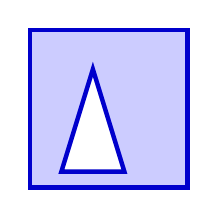
\begin{tikzpicture}
        % Cuadrado de lado 2 centrado en (0,0) -> de -1,-1 a 1,1
        \fill[blue!20] (-1,-1) rectangle (1,1);
        \draw[blue!80!black, ultra thick] (-1,-1) rectangle (1,1);
        
        % Triángulo inscrito (aproximado según la figura del pdf)
        % Base en la parte inferior, pico arriba pero no centrado completamente o quizás sí.
        % En la figura original el triángulo es isosceles estrecho desplazado a la izquierda.
        % Simulamos la apariencia visual del problema 5.1 (figura página 58)
        \coordinate (A) at (-0.5, -0.8);
        \coordinate (B) at (0.0, 0.2);
        \coordinate (C) at (0.5, -0.8);
        % Ajustando para que parezca el de la diapositiva (triángulo blanco borde azul)
        \fill[white] (-0.6, -0.8) -- (-0.2, 0.5) -- (0.2, -0.8) -- cycle;
        \draw[blue!80!black, ultra thick] (-0.6, -0.8) -- (-0.2, 0.5) -- (0.2, -0.8) -- cycle;
    \end{tikzpicture}
    \end{center}
\end{ejercicio}

\begin{solucion} Solución al problema 5.1:
    \lstinputlisting{../code/EjerciciosTeoria/problema_5_1.gd}
\end{solucion}

\begin{ejercicio}
    % \textbf{Proyecto con dos escenas}

    Crea un proyecto Godot con una escena principal con un nodo raíz compuesto. Ese nodo tendrá tres hijos, cada uno es una instancia de la escena del problema anterior, pero con una transformación distinta.

    \begin{center}
    % \begin{tikzpicture}[line width=1.5pt, blue, fill=blue!20]
    %     % Definición de coordenadas base
    %     % Cuadrado de la izquierda (1x1)
    %     \draw [fill] (0,0) rectangle (1.5,1.5);
    %     \draw [white, fill=white] (0.15,0.2) -- (0.45,0.2) -- (0.35,1) -- cycle;

    %     % Rombo central (Cuadrado rotado 45 grados)
    %     % El vértice izquierdo del rombo toca el vértice superior derecho del primer cuadrado (1.5, 1.5)
    %     % El lado del rombo es aproximadamente 2.12 para que sus extremos conecten bien
    %     \begin{scope}[shift={(3, 1.5)}, rotate=45]
    %         \draw [fill] (-1.06,-1.06) rectangle (1.06,1.06);
    %         % Triángulo apuntando hacia arriba dentro del rombo
    %         \draw [white, fill=white] (0,0.5) -- (-0.4,-0.2) -- (0.4,-0.2) -- cycle;
    %     \end{scope}

    %     % Rectángulo de la derecha
    %     % Empieza donde termina el rombo en el eje x (4.5)
    %     \draw [fill] (4.5,0) rectangle (7.5,1.5);
    %     \draw [white, fill=white] (4.8, 1.3) -- (5.8, 1.3) -- (5.3, 0.5) -- cycle;
    % \end{tikzpicture}
    \begin{center}
        \includegraphics[width=0.8\textwidth]{../media/ej5-2.png}
    \end{center}
    \end{center}
\end{ejercicio}

\begin{solucion} Solución al problema 5.2:
    \lstinputlisting{../code/EjerciciosTeoria/problema_5_2.gd}
\end{solucion}

\begin{ejercicio}
    % \textbf{Escena simple: Tronco}

    Implementa un proyecto Godot con una función \texttt{Tronco} que crea y devuelve un \texttt{Node2D} con dos nodos hijos que forman la figura de aquí abajo (uno para el relleno y otro para las aristas).

    Tabla de coordenadas:
    \begin{center}
    \begin{tabular}{c c}
        0 & $(+0.0, +0.0)$ \\
        1 & $(+1.0, +0.0)$ \\
        2 & $(+1.0, +1.0)$ \\
        3 & $(+2.0, +2.0)$ \\
        4 & $(+1.5, +2.5)$ \\
        5 & $(+0.5, +1.5)$ \\
        6 & $(+0.0, +3.0)$ \\
        7 & $(-0.5, +3.0)$ \\
        8 & $(+0.0, +1.5)$ \\
    \end{tabular}
    \end{center}

    \begin{center}
    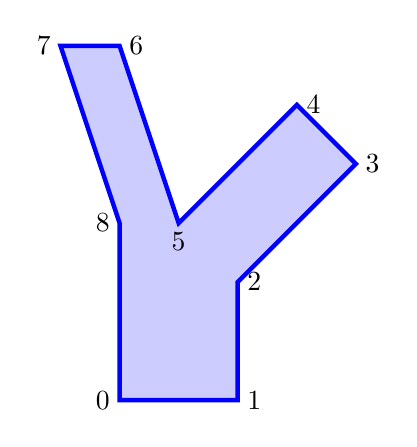
\begin{tikzpicture}[scale=1.5]
        \coordinate (P0) at (0.0, 0.0);
        \coordinate (P1) at (1.0, 0.0);
        \coordinate (P2) at (1.0, 1.0);
        \coordinate (P3) at (2.0, 2.0);
        \coordinate (P4) at (1.5, 2.5);
        \coordinate (P5) at (0.5, 1.5);
        \coordinate (P6) at (0.0, 3.0);
        \coordinate (P7) at (-0.5, 3.0);
        \coordinate (P8) at (0.0, 1.5);

        % Relleno
        \fill[blue!20] (P0) -- (P1) -- (P2) -- (P3) -- (P4) -- (P5) -- (P6) -- (P7) -- (P8) -- cycle;
        % Aristas
        \draw[blue, ultra thick] (P0) -- (P1) -- (P2) -- (P3) -- (P4) -- (P5) -- (P6) -- (P7) -- (P8) -- cycle;

        % Etiquetas de vértices
        \node[left] at (P0) {0};
        \node[right] at (P1) {1};
        \node[right] at (P2) {2};
        \node[right] at (P3) {3};
        \node[right] at (P4) {4};
        \node[below] at (P5) {5};
        \node[right] at (P6) {6};
        \node[left] at (P7) {7};
        \node[left] at (P8) {8};
    \end{tikzpicture}
    \end{center}
\end{ejercicio}

\begin{solucion} Solución al problema 5.3:
    \lstinputlisting{../code/EjerciciosTeoria/problema_5_3.gd}
\end{solucion}

\begin{ejercicio}
    % \textbf{Figura recursiva}

    Implementa otro proyecto Godot que use la función del problema anterior para otra función, \texttt{Arbol(n)}, que genera un árbol de escena con la figura de aquí abajo, que incluye múltiples instancias de \texttt{Tronco}, situadas recursivamente unas adyacentes a otras, hasta un nivel de recursividad dado por $n$.

\end{ejercicio}

\begin{solucion} Solución al problema 5.4:
    \lstinputlisting{../code/EjerciciosTeoria/problema_5_4.gd}
\end{solucion}

\begin{ejercicio}
    % \textbf{Árbol de escena 3D}

    En un proyecto Godot 3D (puedes usar la práctica 2), crea una figura como el logo de Android, usando únicamente dos objetos \texttt{ArrayMesh}, uno con un cilindro y otro con una semiesfera.

    \begin{center}
    
\begin{tikzpicture}
        % Representación esquemática del logo de Android
        \definecolor{androidgreen}{RGB}{164, 198, 57}
        
        % Cuerpo (Cilindro simplificado como rectángulo con base curva)
        \fill[androidgreen] (-1.2, 0) -- (1.2, 0) -- (1.2, -2.5) arc(0:-180:0.2 and 0.1) -- (-1.2, -2.5) -- cycle;
        \fill[androidgreen] (-1.2, -2.5) arc(180:360:1.2 and 0.2); % Base redondeada
        
        % Cabeza (Semiesfera)
        \fill[androidgreen] (0, 0.2) circle [x radius=1.25, y radius=1.0, start angle=0, end angle=180];
        \fill[white] (-1.3, 0.2) rectangle (1.3, -0.1); % Cortar la parte de abajo para hacerla plana (gap)
        \fill[androidgreen] (1.25, 0.2) arc(0:180:1.25);
        
        % Ojos
        \fill[white] (-0.5, 0.8) circle (0.12);
        \fill[white] (0.5, 0.8) circle (0.12);
        
        % Antenas
        \draw[androidgreen, line width=3pt, line cap=round] (-0.6, 1.2) -- (-0.9, 1.7);
        \draw[androidgreen, line width=3pt, line cap=round] (0.6, 1.2) -- (0.9, 1.7);
        
        % Brazos (Cilindros con terminaciones esféricas)
        \fill[androidgreen, rounded corners=5pt] (-1.8, 0.1) rectangle (-1.4, -1.8);
        \fill[androidgreen, rounded corners=5pt] (1.4, 0.1) rectangle (1.8, -1.8);
        
        % Piernas (Cilindros)
        \fill[androidgreen, rounded corners=5pt] (-0.8, -2.2) rectangle (-0.4, -3.2);
        \fill[androidgreen, rounded corners=5pt] (0.4, -2.2) rectangle (0.8, -3.2);

    \end{tikzpicture}
    \end{center}
    \begin{center}
        \includegraphics[width=0.5\textwidth]{../media/android-logo.png}
    \end{center}
\end{ejercicio}

\begin{solucion} Solución al problema 5.5:
    \lstinputlisting{../code/EjerciciosTeoria/problema_5_5.gd}
\end{solucion}



\section{Sesión 6}

\begin{ejercicio}

Escribe el código GDScript para adjuntar a un nodo de tipo Camera3D, de forma que en cada frame la cámara apunte a un objeto móvil objetivo (por ejemplo un coche), con estos requerimientos:
\begin{itemize}
    \item La posición y el vector de velocidad del objetivo (en coordenadas de mundo) se pueden obtener con dos funciones globales, llamadas \texttt{objetivo.posicion()} y \texttt{objetivo.velocidad()}, ambas devuelven un objeto de tipo \texttt{Vector3}.
    \item La cámara debe situarse detrás del objetivo, de forma que el punto devuelto por \texttt{objetivo.posicion()} se proyecte en el centro del viewport, y además la cámara esté situada 3 unidades en horizontal por detrás del objetivo, y 2 unidades por encima (en el eje Y).
\end{itemize}
\end{ejercicio}

\begin{solucion} Nuestro objetivo móvil va a ser un coche. La resolución detallada es la siguiente:\\

\subsubsection*{Requerimientos Geométricos:}

\begin{enumerate}
    \item \textbf{Punto de Atención (Look At):} La cámara debe apuntar al objetivo. Esto significa que el eje $-Z$ de la cámara (en Godot, la cámara ''mira'' hacia $-Z$ local) debe alinearse con el vector que va desde la cámara hasta el objetivo. El punto $\vec{p}_{obj}$ se proyectará en el centro del \emph{viewport}.
    \item \textbf{Posición Relativa:}
    \begin{itemize}
        \item \textbf{''Detrás'' (Horizontal):} 3 unidades por detrás. ''Detrás'' se define en relación con el movimiento. Si el coche se mueve hacia adelante, ''detrás'' es la dirección opuesta a la velocidad. Debemos considerar solo la componente horizontal para evitar que la cámara se incline hacia el suelo si el coche sube una pendiente.
        \item \textbf{''Arriba'' (Vertical):} 2 unidades por encima del objetivo (eje Y global).
    \end{itemize}
\end{enumerate}

\subsubsection*{Fundamentación Teórica}

Para resolver esto, utilizamos conceptos de \textbf{Espacios Afines} y \textbf{Operaciones con Vectores} (tratados en el pdf \texttt{ig-s03.pdf}):

\begin{enumerate}
    \item \textbf{Definición de ''Atrás'':}
    El vector velocidad $\vec{v}_{obj}$ nos da la dirección del movimiento. Para situarnos ''detrás'' horizontalmente:
    \begin{itemize}
        \item Tomamos $\vec{v}_{obj}$ y anulamos su componente Y (para que sea puramente horizontal): $\vec{d}_{hz} = (v_x, 0, v_z)$.
        \item Normalizamos este vector para obtener una dirección unitaria: $\hat{d}_{hz} = \vec{d}_{hz} / |\vec{d}_{hz}|$.
        \item El vector ''hacia atrás'' es $-\hat{d}_{hz}$.
        \item El desplazamiento horizontal deseado es $-3 \cdot \hat{d}_{hz}$.
    \end{itemize}
    \item \textbf{Composición de la Posición de la Cámara ($\vec{p}_{cam}$):}
    \[
        \vec{p}_{cam} = \vec{p}_{obj} + (0,2,0) - 3 \cdot \hat{d}_{hz}
    \]
    Donde:
    \begin{itemize}
        \item $(0,2,0)$: 2 unidades arriba.
        \item $-3 \cdot \hat{d}_{hz}$: 3 unidades atrás.
    \end{itemize}
    \item \textbf{Transformación de Vista (LookAt):}
    Una vez tenemos $\vec{p}_{cam}$, necesitamos construir la matriz de vista. En Godot, la clase \texttt{Node3D} (de la cual hereda \texttt{Camera3D}) tiene métodos auxiliares para esto. El método \texttt{look\_at(target, up)} ajusta la transformación del nodo para que mire a \texttt{target} manteniendo el vector \texttt{up} orientado hacia arriba tanto como sea posible.
\end{enumerate}

\subsubsection*{Solución: Código GDScript}

\begin{lstlisting}[language=gdscript]
extends Camera3D

# Asumimos que 'objetivo' es un singleton (AutoLoad) o una clase global accesible.
# Si no fuera global, habría que obtener la referencia al nodo (ej. get_node(''../Coche''))

func _process(delta: float):
    # 1. Obtener datos del objetivo (en coordenadas de mundo)
    # Según el enunciado, existen estas funciones globales.
    var p_obj: Vector3 = objetivo.posicion()
    var v_obj: Vector3 = objetivo.velocidad()
    
    # 2. Calcular la dirección horizontal del movimiento
    # Creamos un vector con la velocidad pero ignorando la componente Y
    var direccion_hz: Vector3 = Vector3(v_obj.x, 0.0, v_obj.z)
    
    # IMPORTANTE: Si el coche está parado (velocidad casi 0), no podemos normalizar 
    # (división por cero). En un caso real, mantendríamos la última dirección válida.
    # Para el ejercicio, asumimos movimiento o usamos una dirección por defecto (ej. eje Z).
    if direccion_hz.length_squared() > 0.001:
        direccion_hz = direccion_hz.normalized()
    else:
        # Fallback: si está quieto, asumimos que ''detrás'' es el eje Z positivo (por ejemplo)
        # O idealmente, usaríamos la orientación del nodo objetivo (basis.z)
        direccion_hz = Vector3(0, 0, 1) 

    # 3. Calcular la posición deseada de la cámara
    # - Situada en la posición del objetivo
    # - Desplazada 2 unidades hacia ARRIBA (Eje Y global)
    # - Desplazada 3 unidades hacia ATRÁS (opuesto a la dirección horizontal)
    var nueva_posicion: Vector3 = p_obj + Vector3(0, 2, 0) - (direccion_hz * 3.0)
    
    # 4. Aplicar la posición a la cámara
    # Usamos global_position para asegurar que estamos en coords de mundo
    global_position = nueva_posicion
    
    # 5. Orientar la cámara (Transformación de Vista)
    # Hacemos que la cámara mire al punto objetivo.
    # El vector ''Arriba'' (Up) suele ser el eje Y global (Vector3.UP)
    look_at(p_obj, Vector3.UP)
\end{lstlisting}

\subsubsection*{Explicación detallada de la implementación}

\begin{enumerate}
    \item \textbf{\texttt{extends Camera3D}}: El script hereda de la clase base de cámaras en Godot, permitiendo controlar la proyección y vista.
    \item \textbf{\texttt{\_process(delta)}}: Usamos este método del bucle principal (\texttt{MainLoop}) porque el enunciado pide que la cámara se actualice ''en cada frame''.
    \item \textbf{Cálculo del vector dirección}:
    \begin{itemize}
        \item El enunciado especifica ''3 unidades en horizontal''. Esto es crucial. Si usáramos el vector velocidad completo (incluyendo Y) para calcular el ''atrás'', y el coche subiera una rampa muy empinada, la cámara se metería bajo tierra. Por eso proyectamos sobre el plano XZ haciendo $v_{obj}.y = 0$ y luego normalizamos $v.normalized()$.
    \end{itemize}
    \item \textbf{Posicionamiento (\texttt{global\_position})}:
    \begin{itemize}
        \item Calculamos la posición final sumando vectores. Matemáticamente: $\vec{p}_{cam} = \vec{p}_{obj} + (0,2,0) - 3 \cdot \hat{d}_{hz}$.
    \end{itemize}
    \item \textbf{Orientación (\texttt{look\_at})}:
    \begin{itemize}
        \item Este método es fundamental en la \textbf{Transformación de Vista}. Recalcula la matriz de transformación del nodo (\texttt{transform}) para que su eje $-Z$ (visión) apunte a $\vec{p}_{obj}$ y su eje $Y$ se alinee con \texttt{Vector3.UP}. Esto resuelve la parte compleja de crear la matriz de rotación ortonormal manualmente.
    \end{itemize}
\end{enumerate}

\end{solucion}

\begin{ejercicio}
Supongamos una escena que contiene una representación visible del marco de coordenadas del mundo como tres flechas (roja X, verde Y y azul Z), como ocurre en las prácticas. Queremos visualizar esa escena en pantalla, de forma que:
\begin{enumerate}
    \item El eje Y aparezca vertical, hacia arriba, el eje X horizontal, hacia la derecha, el eje Z horizontal, hacia la izquierda (los ejes X y Z se visualizan con la misma longitud aparente).
    \item El punto de coordenadas $(0, 0.5, 0)$ (aparece como un disco de color morado en la figura) debe aparecer en el centro del viewport.
    \item El observador (foco de la proyección) estará a 3 unidades de distancia del punto $(0, 0.5, 0)$.
\end{enumerate}

Escribe unos valores que podríamos usar para $\mathbf{a}$, $\mathbf{u}$ y $\mathbf{n}$ de forma que se cumplan estos requisitos. En la figura se observa una vista esquemática de cómo quedaría la figura en un viewport cuadrado.

\begin{center}
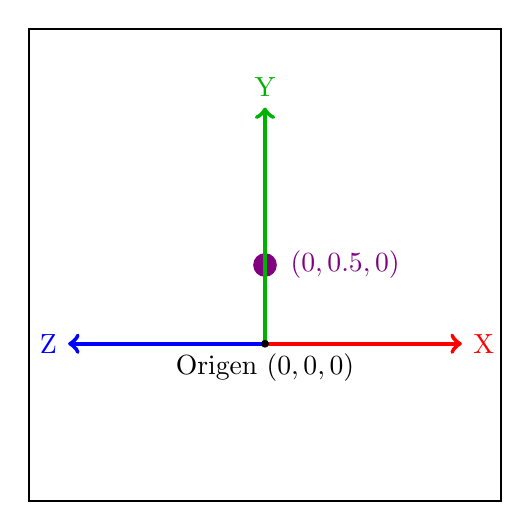
\begin{tikzpicture}
    % Viewport frame
    \draw[thick] (-3,-3) rectangle (3,3);
    
    % Origin point (approximate projection below center)
    \coordinate (O) at (0, -1);
    
    % Center point (a)
    \coordinate (A) at (0, 0); 
    \fill[violet] (A) circle (0.15);
    \node[right, violet] at (0.2, 0) {$(0, 0.5, 0)$};
    
    % Axes
    % Y axis (Green, Up)
    \draw[->, ultra thick, green!70!black] (O) -- (0, 2) node[above] {Y};
    
    % X axis (Red, Right)
    \draw[->, ultra thick, red] (O) -- (2.5, -1) node[right] {X};
    
    % Z axis (Blue, Left)
    \draw[->, ultra thick, blue] (O) -- (-2.5, -1) node[left] {Z};
    
    % Origin dot
    \fill[black] (O) circle (0.05);
    \node[below] at (O) {Origen $(0,0,0)$};
    
\end{tikzpicture}
\hspace{1cm}
\includegraphics[height=6cm]{../media/p6-2.png}
\end{center}
\end{ejercicio}

\begin{solucion}
Para determinar los parámetros de la matriz de vista ($\mathbf{a}$, $\mathbf{u}$, $\mathbf{n}$), analizamos cada requerimiento paso a paso:

\begin{enumerate}
    \item \textbf{Determinación del punto de atención ($\mathbf{a}$):}
    El enunciado establece que el punto de coordenadas $(0, 0.5, 0)$ debe aparecer en el centro del viewport. Por definición, el punto de atención $\mathbf{a}$ (Look-At point) es el punto hacia el que apunta la cámara y que se proyecta en el centro del plano de imagen.
    
    Por lo tanto:
    \[ \mathbf{a} = (0, 0.5, 0) \]

    \item \textbf{Determinación del vector hacia arriba ($\mathbf{u}$):}
    Se requiere que el eje Y del mundo aparezca vertical y hacia arriba en la imagen. Dado que el eje Y del mundo es $(0, 1, 0)$, la forma más directa de conseguir que se proyecte verticalmente es alineando el vector \textit{view-up} ($\mathbf{u}$) con el eje Y del mundo (siempre que la dirección de vista no sea paralela a este eje, lo cual verificaremos en el siguiente paso).
    
    Por lo tanto:
    \[ \mathbf{u} = (0, 1, 0) \]

    \item \textbf{Determinación del vector normal de vista ($\mathbf{n}$):}
    El vector $\mathbf{n}$ define la dirección desde el punto de atención hacia el observador (es decir, la inversa de la dirección de la vista). También determina la posición del observador $\mathbf{o}_{ec}$ mediante la relación $\mathbf{o}_{ec} = \mathbf{a} + \mathbf{n}$.
    
    Analizamos las condiciones para $\mathbf{n} = (n_x, n_y, n_z)$:
    \begin{itemize}
        \item \textbf{Longitud:} El observador debe estar a 3 unidades de distancia de $\mathbf{a}$. Como $\mathbf{n}$ es el vector que une $\mathbf{a}$ con el observador, su norma debe ser 3:
        \[ ||\mathbf{n}|| = 3 \]
        
        \item \textbf{Orientación Horizontal:} Para que el eje Y se vea perfectamente vertical y centrado, la cámara debe estar a la misma altura o el vector de visión debe estar contenido en un plano vertical que contenga al eje Y. Sin embargo, la condición crítica proviene de los ejes X y Z.
        
        \item \textbf{Orientación de X y Z:}
        \begin{itemize}
            \item El eje X debe verse horizontal hacia la derecha.
            \item El eje Z debe verse horizontal hacia la izquierda.
            \item Ambos deben tener la misma longitud aparente.
        \end{itemize}
        
        Esto implica que el observador debe situarse en una posición simétrica respecto a los ejes X e Z positivos (primer cuadrante del plano XZ respecto a $\mathbf{a}$), de forma que la línea de visión biseque el ángulo de 90 grados entre X y Z.
        
        Si nos situamos en la bisectriz del primer cuadrante del plano XZ, el vector de dirección tendrá componentes X y Z iguales y positivas. El eje X (derecha) y el eje Z (adelante) formarán ambos un ángulo de $45^\circ$ con el plano de proyección, proyectándose hacia lados opuestos (derecha e izquierda) con la misma deformación (longitud aparente).
        
        Por tanto, la dirección de $\mathbf{n}$ debe ser $(1, 0, 1)$.
    \end{itemize}
    
    Calculamos $\mathbf{n}$:
    \begin{enumerate}
        \item Tomamos el vector director base: $\vec{d} = (1, 0, 1)$.
        \item Calculamos su norma: $||\vec{d}|| = \sqrt{1^2 + 0^2 + 1^2} = \sqrt{2}$.
        \item Normalizamos y escalamos por la distancia requerida (3 unidades):
        \[ \mathbf{n} = 3 \cdot \frac{\vec{d}}{||\vec{d}||} = 3 \cdot \frac{(1, 0, 1)}{\sqrt{2}} = \left( \frac{3}{\sqrt{2}}, 0, \frac{3}{\sqrt{2}} \right) \]
    \end{enumerate}
    
    Aproximando los valores:
    \[ \frac{3}{\sqrt{2}} = \frac{3 \sqrt{2}}{2} \approx 2.1213 \]
    
    Así, $\mathbf{n} \approx (2.12, 0, 2.12)$.
\end{enumerate}

\textbf{Resultado Final:}
Los valores que cumplen los requisitos son:
\[ \mathbf{a} = (0, 0.5, 0) \]
\[ \mathbf{u} = (0, 1, 0) \]
\[ \mathbf{n} = \left( \frac{3}{\sqrt{2}}, 0, \frac{3}{\sqrt{2}} \right) \]

\end{solucion}

\begin{ejercicio}
Repite el problema anterior 6.2, pero ahora para esta vista (ver figura). Usa una rotación del marco de vista entorno a uno de sus propios ejes.

\begin{center}
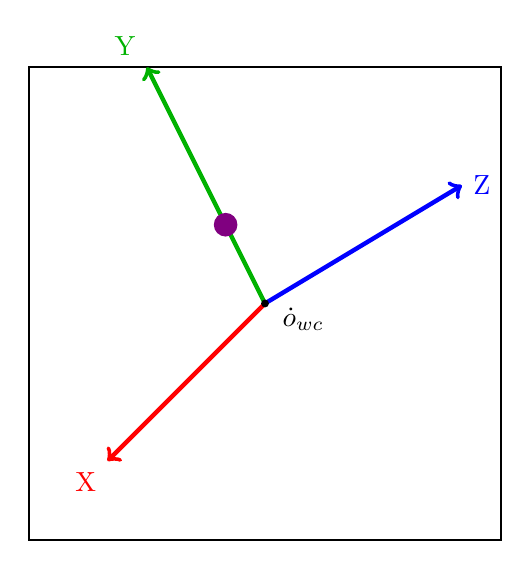
\begin{tikzpicture}
    % Viewport frame
    \draw[thick] (-3,-3) rectangle (3,3);
    
    % Origin point (black dot)
    \coordinate (O) at (0, 0);
    
    % Center point a (purple dot on Y axis)
    \coordinate (A) at (-0.5, 1); 
    
    % Axes visual representation based on Image 6.3
    % Y axis (Green, Up-Left)
    \draw[->, ultra thick, green!70!black] (O) -- (-1.5, 3) node[above left] {Y};
    \fill[violet] (A) circle (0.15); % Point a
    
    % Z axis (Blue, Up-Right)
    \draw[->, ultra thick, blue] (O) -- (2.5, 1.5) node[right] {Z};
    
    % X axis (Red, Down-Left)
    \draw[->, ultra thick, red] (O) -- (-2, -2) node[below left] {X};
    
    % Origin dot
    \fill[black] (O) circle (0.05);
    \node[right] at (0.1, -0.2) {$\dot{o}_{wc}$};
    
\end{tikzpicture}
\hspace{1cm}
\includegraphics[height=6cm]{../media/p6-3.png}
\end{center}

Escribe los valores para $\mathbf{a}$, $\mathbf{u}$ y $\mathbf{n}$.
\end{ejercicio}

\begin{solucion}
Para obtener la configuración visual mostrada en la figura, partimos de la solución del ejercicio 6.2 y aplicamos las transformaciones necesarias.

\begin{enumerate}
    \item \textbf{Punto de atención ($\mathbf{a}$):}
    Al igual que en el ejercicio anterior, el punto $(0, 0.5, 0)$ (disco morado) debe aparecer en el centro del viewport. Por tanto:
    \[ \mathbf{a} = (0, 0.5, 0) \]

    \item \textbf{Vector normal de vista ($\mathbf{n}$):}
    Observamos la orientación de los ejes X y Z:
    \begin{itemize}
        \item El eje X (rojo) apunta hacia la izquierda y abajo.
        \item El eje Z (azul) apunta hacia la derecha y arriba.
    \end{itemize}
    En el ejercicio 6.2, mirábamos desde el primer cuadrante $(+X, +Z)$, viendo el eje X a la derecha y Z a la izquierda. Aquí la situación horizontal se ha invertido (X a la izquierda, Z a la derecha), lo que implica que el observador se ha movido a la posición opuesta (''detrás'' de la escena), mirando desde el cuadrante $(-X, -Z)$.
    
    El vector de dirección base sería $(-1, 0, -1)$. Normalizando y aplicando la distancia de 3 unidades:
    \[ \mathbf{n} = 3 \cdot \frac{(-1, 0, -1)}{\sqrt{(-1)^2 + 0^2 + (-1)^2}} = 3 \cdot \left( \frac{-1}{\sqrt{2}}, 0, \frac{-1}{\sqrt{2}} \right) \]
    
    Aproximando:
    \[ \mathbf{n} \approx (-2.12, 0, -2.12) \]

    \item \textbf{Vector hacia arriba ($\mathbf{u}$):}
    Observamos el eje Y (verde). En lugar de apuntar verticalmente hacia arriba (como haría con $\mathbf{u}=(0,1,0)$), apunta hacia arriba a la izquierda. Esto indica una rotación de la cámara (Roll) alrededor del eje de visión $\mathbf{n}$.
    
    Si usáramos $\mathbf{u}_{base} = (0,1,0)$ desde la posición trasera, veríamos el eje Y vertical. Para que el eje Y se incline hacia la izquierda en la pantalla, la cámara debe rotar en sentido horario (CW). Una rotación de 45 grados en sentido horario del vector $\mathbf{u}_{base}$ alrededor del eje de visión nos da el vector necesario.
    
    Calculamos $\mathbf{u}$ como una combinación lineal que se incline hacia el eje Z negativo y X negativo (para mantener la ortogonalidad con $\mathbf{n}$):
    \[ \mathbf{u} = (-1, 1, 1) \]
    (Nota: Se puede normalizar a $(-1/\sqrt{3}, 1/\sqrt{3}, 1/\sqrt{3})$).
    
    Verificación rápida: $\mathbf{n} \cdot \mathbf{u} = (-1)(-1) + (0)(1) + (-1)(1) = 1 + 0 - 1 = 0$. Son perpendiculares.

    \vspace{1em}
    \textbf{¿Cómo se calcula $\mathbf{u}$ exactamente?}

    El vector $\mathbf{u}$ (View-Up) indica la dirección de ''arriba'' para la cámara. El procedimiento ordenado para deducir $\mathbf{u} = (-1, 1, 1)$ es:

    \begin{enumerate}
        \item \textbf{Definir la base sin rotar:}
        \begin{itemize}
            \item Nos situamos ''detrás'' de la escena (lado opuesto al ejercicio 6.2), ya que el eje X va a la izquierda y el Z a la derecha.
            \item Vector de vista ideal: $\mathbf{n} = (-1, 0, -1)$.
            \item Vector arriba estándar: $\mathbf{u}_{base} = (0, 1, 0)$.
        \end{itemize}
        \item \textbf{Calcular el vector ''Derecha'':}
        \[
            \text{Derecha} = \mathbf{u}_{base} \times \mathbf{n} = (0, 1, 0) \times (-1, 0, -1) = (-1, 0, 1)
        \]
        Sabemos que $\text{Arriba} \times \text{Atrás} = \text{Derecha}$. Para el caso de la izquierda sería el opuesto. (n es atrás y u es arriba).
        \item \textbf{Aplicar la rotación (mezclar arriba y derecha):}
        \begin{itemize}
            \item Para rotar la cámara hacia la derecha (sentido horario), sumamos el vector arriba original y el vector derecha:
            \[
                \mathbf{u} = \mathbf{u}_{base} + \text{Derecha} = (0, 1, 0) + (-1, 0, 1) = (-1, 1, 1)
            \]
            \item Este vector tiene componente en Y (arriba), pero también en X y Z, inclinando el ''arriba'' de la cámara hacia la derecha de la pantalla, logrando el efecto de rotación deseado.
        \end{itemize}
    \end{enumerate}


\end{enumerate}

\textbf{Valores Finales:}
\[ \mathbf{a} = (0, 0.5, 0) \]
\[ \mathbf{u} = (-1, 1, 1) \quad (\text{o normalizado } \approx (-0.577, 0.577, 0.577)) \]
\[ \mathbf{n} = \left( \frac{-3}{\sqrt{2}}, 0, \frac{-3}{\sqrt{2}} \right) \approx (-2.12, 0, -2.12) \]

\end{solucion}

\begin{ejercicio}
Escribe el código GDScript para calcular los vectores de coordenadas $o_{ec}$, $x_{ec}$, $y_{ec}$ y $z_{ec}$ que definen el marco de vista a partir de los vectores de coordenadas $a$, $u$ y $n$ (todos estos vectores de coordenadas de mundo, en objetos de tipo Vector3).
\end{ejercicio}

\begin{solucion}
Para construir el marco de referencia de vista (view reference frame) a partir de los vectores dados, seguimos el procedimiento estándar de la transformación de cámara en gráficos 3D:

\begin{enumerate}
    \item \textbf{Cálculo del origen del marco ($o_{ec}$):}
    El origen del marco de cámara (posición del observador) se obtiene sumando el punto de atención $a$ y el vector normal $n$:
    \[
        o_{ec} = a + n
    \]

    \item \textbf{Cálculo del eje $z_{ec}$:}
    El eje $z_{ec}$ es la dirección de la vista (normalizada) y se obtiene normalizando el vector $n$:
    \[
        z_{ec} = \frac{n}{\|n\|}
    \]

    \item \textbf{Cálculo del eje $x_{ec}$:}
    El eje $x_{ec}$ (derecha de la cámara) se obtiene como el producto vectorial entre el vector hacia arriba $u$ y el vector normal $n$, normalizado:
    \[
        x_{ec} = \frac{u \times n}{\|u \times n\|}
    \]

    \item \textbf{Cálculo del eje $y_{ec}$:}
    El eje $y_{ec}$ (arriba de la cámara) se obtiene como el producto vectorial entre $z_{ec}$ y $x_{ec}$:
    \[
        y_{ec} = z_{ec} \times x_{ec}
    \]
\end{enumerate}

El siguiente código GDScript implementa estos pasos, suponiendo que $a$, $u$ y $n$ son objetos de tipo \texttt{Vector3}:

\begin{lstlisting}
# a, u, n: Vector3 (coordenadas de mundo)

# 1. Origen del marco de cámara
var o_ec : Vector3 = a + n

# 2. Eje Z (dirección de la vista, normalizado)
var z_ec : Vector3 = n.normalized()

# 3. Eje X (derecha, ortogonal a u y n, normalizado)
var x_ec : Vector3 = u.cross(n).normalized()

# 4. Eje Y (arriba, ortogonal a z_ec y x_ec)
var y_ec : Vector3 = z_ec.cross(x_ec)
\end{lstlisting}

Este procedimiento garantiza que los vectores $x_{ec}$, $y_{ec}$ y $z_{ec}$ forman una base ortonormal adecuada para definir el sistema de referencia de la cámara.
\end{solucion}

\begin{ejercicio}
Partiendo de los vectores de coordenadas $o_{ec}$, $x_{ec}$, $y_{ec}$ y $z_{ec}$ que se calculan en el problema anterior, escribe el código que calcula explícitamente la matriz de vista, es una variable de tipo \texttt{Transform3D}.
\end{ejercicio}

\begin{solucion}
Para construir la matriz de vista (\textit{View Matrix}) a partir del marco de cámara definido por $o_{ec}$ (origen), $x_{ec}$, $y_{ec}$ y $z_{ec}$ (vectores ortonormales), seguimos el procedimiento estándar de gráficos 3D:

\begin{enumerate}
    \item \textbf{Definición:} La matriz de vista transforma coordenadas del mundo al sistema de la cámara. Se compone de una rotación (alineando los ejes del mundo con los de la cámara) y una traslación (llevando el origen de la cámara al origen del sistema).
    \item \textbf{Expresión matricial:}
    \[
    V = \begin{pmatrix}
    x_{ec}.x & x_{ec}.y & x_{ec}.z & -(x_{ec} \cdot o_{ec}) \\
    y_{ec}.x & y_{ec}.y & y_{ec}.z & -(y_{ec} \cdot o_{ec}) \\
    z_{ec}.x & z_{ec}.y & z_{ec}.z & -(z_{ec} \cdot o_{ec}) \\
    0 & 0 & 0 & 1
    \end{pmatrix}
    \]
    \item \textbf{Implementación en Godot (\texttt{Transform3D}):}
    En Godot, la clase \texttt{Transform3D} almacena la base (rotación) y el origen (traslación). La base se define por columnas, por lo que debemos transponer la matriz formada por $x_{ec}$, $y_{ec}$ y $z_{ec}$ como filas.
\end{enumerate}

\hspace{1cm}

\textbf{Código GDScript:}
\begin{lstlisting}
# Suponemos disponibles: x_ec, y_ec, z_ec, o_ec (Vector3)

# 1. Construir la base (rotación): columnas de la base son los ejes de cámara
var R := Basis(x_ec, y_ec, z_ec)
var vista_basis := R.transposed()

# 2. Calcular la traslación (origen) según la fórmula de la matriz de vista
var d_x = -x_ec.dot(o_ec)
var d_y = -y_ec.dot(o_ec)
var d_z = -z_ec.dot(o_ec)
var vista_origin = Vector3(d_x, d_y, d_z)

# 3. Construir la matriz de vista final
var matriz_vista = Transform3D(vista_basis, vista_origin)

# La función de Transform3D lo que es empaqueta todo en un solo objeto, en este caso, lo que hace es crear una matriz de 4x4 a partir de una matriz de 3x3 (Basis) y un vector de traslación (origin).
\end{lstlisting}

\textbf{Explicación:} La matriz de vista es la inversa de la transformación de la cámara en el mundo. La base ortonormal se transpone para invertir la rotación, y la traslación se obtiene proyectando el origen del marco de cámara sobre cada eje y cambiando el signo, lo que equivale a trasladar el mundo al sistema de la cámara. Usamos cross para construir el marco de referencia, y dot para situar puntos dentro de ese marco, en este caso como lo que se busca es \underline{proyectar usamos dot}.
\end{solucion}

\begin{ejercicio}

En una copia independiente del código de prácticas, modifica el nodo de la cámara orbital simple para conseguir que el fov mínimo (vertical u horizontal) sea siempre de $75^{\circ}$. Esto servirá, por ejemplo, para ver el cubo de las prácticas siempre completo independientemente del ancho y alto de la ventana.

Para ello:
\begin{enumerate}
    \item Añadir al script del nodo de cámara una función que se ejecute siempre que se redimensione la ventana (y al inicio).
    \item En esa función, obtener el tamaño (alto y ancho) del viewport.
    \item Calcular la relación de aspecto ($ancho/alto$).
    \item Usar ajuste de la proyección en vertical si el viewport es más ancho que alto, y ajuste en horizontal en caso contrario.
\end{enumerate}

\begin{center}
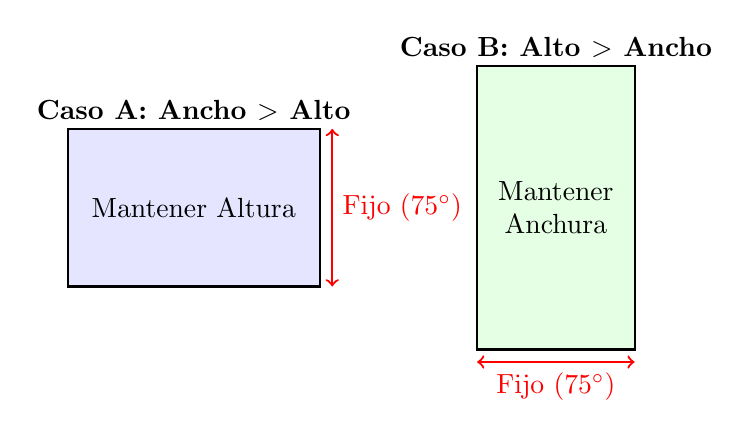
\begin{tikzpicture}[scale=0.8]
    % Escenario 1: Landscape (Ancho > Alto)
    \draw[thick, fill=blue!10] (0,0) rectangle (4, 2.5);
    \node at (2, 2.8) {\textbf{Caso A: Ancho $>$ Alto}};
    \node at (2, 1.25) {Mantener Altura};
    \draw[<->, red, thick] (4.2, 0) -- (4.2, 2.5) node[midway, right] {Fijo ($75^\circ$)};
    
    % Espacio extra entre los dos escenarios
    \begin{scope}[shift={(6.5,0)}]
        % Escenario 2: Portrait (Alto > Ancho)
        \draw[thick, fill=green!10] (0, -1) rectangle (2.5, 3.5);
        \node at (1.25, 3.8) {\textbf{Caso B: Alto $>$ Ancho}};
        \node[align=center] at (1.25, 1.25) {Mantener\\Anchura};
        \draw[<->, red, thick] (0, -1.2) -- (2.5, -1.2) node[midway, below] {Fijo ($75^\circ$)};
    \end{scope}
\end{tikzpicture}
\end{center}
\end{ejercicio}

\begin{solucion}
Para resolver este problema, debemos manipular la propiedad \texttt{keep\_aspect} de la clase \texttt{Camera3D} en Godot. Esta propiedad determina qué eje (horizontal o vertical) mantiene el ángulo de visión (\texttt{fov}) fijo cuando cambia la relación de aspecto de la ventana.

El objetivo es asegurar que el objeto siempre sea visible. Si la ventana se estrecha horizontalmente, debemos fijar el FOV horizontal. Si se estrecha verticalmente, debemos fijar el FOV vertical.

\begin{enumerate}
    \item \textbf{Lógica del algoritmo:}
    \begin{itemize}
        \item Obtenemos el tamaño del viewport: $w$ (ancho) y $h$ (alto).
        \item Calculamos la relación de aspecto $r = w / h$.
        \item Si $r \geq 1$ (formato apaisado o cuadrado): El ancho es suficiente para contener la escena si fijamos la altura. Usamos \texttt{KEEP\_HEIGHT}.
        \item Si $r < 1$ (formato vertical o ''retrato''): El ancho es el factor limitante. Para evitar que se recorte la escena lateralmente, debemos fijar el ángulo horizontal. Usamos \texttt{KEEP\_WIDTH}.
    \end{itemize}

    \item \textbf{Implementación en GDScript:}
    Añadimos la función \texttt{\_actualiza\_proyeccion} y la conectamos a la señal \texttt{size\_changed} del viewport raíz en la función \texttt{\_ready}.

\begin{lstlisting}
extends Camera3D

# -------------
# constantes y variables de instancia 

const at   := 2.5   # angulo de rot. con teclas
const ar   := 0.5   # angulo de rot. con raton
var   bdrp := false # boton derecho del raton presionado si/no
var   dz   := 3.0   # distancia en Z de la camara al origen
var   dxy  := Vector2( 0.0, 0.0 ) # angulos hor. y vert.

# -------------
# actualiza la variable 'transform' de este nodo camara

func _actualiza_transf_vista(  ) -> void : 
    var ahr  := ((45.0+float(dxy.x))*2.0*PI)/360.0 
    var avr  := ((30.0+float(dxy.y))*2.0*PI)/360.0 
    var tras := Transform3D().translated( Vector3( 0.0, 0.0, dz))   
    var rotx := Transform3D().rotated( Vector3.RIGHT, -avr )
    var roty := Transform3D().rotated( Vector3.UP, ahr ) 
    transform = roty*rotx*tras   

# -------------
# NUEVA FUNCION: Ajuste dinamico de la proyeccion (Problema 6.6)
func _actualiza_proyeccion() -> void:
    # 1. Obtener tamano del viewport
    var vp_size := get_viewport().size
    
    # Evitamos division por cero si la ventana se minimiza completamente
    if vp_size.y == 0: return 

    # 2 y 3. Calcular relacion de aspecto (ancho / alto)
    var aspect_ratio := float(vp_size.x) / float(vp_size.y)
    
    # 4. Ajuste segun la forma de la ventana
    if aspect_ratio < 1.0:
        # Si es mas alto que ancho (Portrait), fijamos el ancho
        keep_aspect = Camera3D.KEEP_WIDTH
    else:
        # Si es mas ancho que alto (Landscape), fijamos el alto (por defecto)
        keep_aspect = Camera3D.KEEP_HEIGHT
        
    # Aseguramos que el FOV base sea siempre 75 grados
    fov = 75.0

# -------------
func _ready() -> void :  
    _actualiza_transf_vista() 
    
    # Conectamos la senal de redimensionado a nuestra nueva funcion
    get_tree().root.size_changed.connect(_actualiza_proyeccion)
    
    # Llamamos a la funcion una vez al inicio para configurar el estado inicial
    _actualiza_proyeccion()
    
# -------------
# procesa evento de entrada (sin cambios respecto al original)

func _input( event : InputEvent ): 
    var av : bool = true 
    
    if event is InputEventKey and event.pressed: 
        match event.keycode:
            KEY_UP:    dxy += Vector2( 0, -at )
            KEY_DOWN:  dxy += Vector2( 0, +at )
            KEY_RIGHT: dxy += Vector2( -at, 0 )
            KEY_LEFT:  dxy += Vector2( at, 0 )
            KEY_MINUS, KEY_PAGEDOWN, KEY_KP_SUBTRACT: dz *= 1.05 
            KEY_PLUS, KEY_PAGEUP, KEY_KP_ADD: dz = max( dz/1.05, 0.1 )
            _: av = false
                
    elif event is InputEventMouseButton: 
        match event.button_index:
            MOUSE_BUTTON_RIGHT: 
                bdrp = event.pressed 
                av = false 
            MOUSE_BUTTON_WHEEL_DOWN: dz *= 1.05
            MOUSE_BUTTON_WHEEL_UP:   dz = max( dz/1.05, 0.1 )
            _: av = false
                
    elif event is InputEventMouseMotion and bdrp: 
        dxy += ar * Vector2( -event.relative.x, event.relative.y ) 
        
    else: 
        av = false 

    if av:
        _actualiza_transf_vista( )
\end{lstlisting}

Para simplificar, lo que se hace es añadir esta función y usarla en el \texttt{\_ready} y cada vez que se redimensiona la ventana:
\begin{lstlisting}[language=GDScript]
# NUEVA FUNCION: Ajuste dinamico de la proyeccion (Problema 6.6)
func _actualiza_proyeccion() -> void:
    # 1. Obtener tamano del viewport
    var vp_size := get_viewport().size
    
    # Evitamos division por cero si la ventana se minimiza completamente
    if vp_size.y == 0: return 

    # 2 y 3. Calcular relacion de aspecto (ancho / alto)
    var aspect_ratio := float(vp_size.x) / float(vp_size.y)
    
    # 4. Ajuste segun la forma de la ventana
    if aspect_ratio < 1.0:
        # Si es mas alto que ancho (Portrait), fijamos el ancho
        keep_aspect = Camera3D.KEEP_WIDTH
    else:
        # Si es mas ancho que alto (Landscape), fijamos el alto (por defecto)
        keep_aspect = Camera3D.KEEP_HEIGHT
        
    # Aseguramos que el FOV base sea siempre 75 grados
    fov = 75.0
\end{lstlisting}
\end{enumerate}
\end{solucion}


% \begin{ejercicio}
% Queremos visualizar una escena con mallas indexadas de la cual sabemos que tiene todos los vértices dentro de un cubo de lado $s$ unidades cuyo centro es el punto de coordenadas del mundo $c=(c_{x},c_{y},c_{z})$. Para construir la matriz de vista, se sitúa el observador en el punto $o_{ec}=(c_{x},c_{y},c_{z}+s+2)$, el punto de atención $a$ se hace igual a $c$ (el centro del cubo se ve en el centro de la imagen), y el vector $u$ es $(0, 1, 0)$. Se visualizará en un viewport cuadrado.

% Queremos construir la matriz de proyección perspectiva $Q$ de forma que se cumplan estos requerimientos:
% \begin{enumerate}
%     \item No se recorta ningún triángulo.
%     \item El tamaño aparente de los objetos (proyectados en pantalla) es el mayor posible.
%     \item El valor del parámetro $n$ es el mayor posible.
%     \item El valor del parámetro $f$ es el menor posible.
%     \item Los objetos no aparecen deformados.
% \end{enumerate}

% Con estos requerimientos, indica cómo calcular los valores $l, r, t, b, n$ y $f$ (para obtener la matriz $Q$ de proyección), en función de $s$ y $c=(c_{x},c_{y},c_{z})$.
% \end{ejercicio}

% \begin{solucion}
% Para resolver este problema, debemos determinar los parámetros del volumen de vista (view frustum) definidos por los planos de recorte: $n$ (near), $f$ (far), $l$ (left), $r$ (right), $b$ (bottom) y $t$ (top). Procederemos analizando la posición de la cámara y la geometría del objeto en el espacio de coordenadas de la cámara (Eye Coordinates, EC).

% \begin{enumerate}
%     \item \textbf{Análisis del Marco de Coordenadas de Vista (EC):}
    
%     Primero determinamos la posición relativa del cubo respecto a la cámara.
%     \begin{itemize}
%         \item \textbf{Posición de la cámara ($E$):} $o_{ec} = (c_x, c_y, c_z + s + 2)$.
%         \item \textbf{Punto de atención ($A$):} $c = (c_x, c_y, c_z)$.
%         \item \textbf{Vector de visión ($\vec{v}$):} $\vec{v} = A - E = (0, 0, -(s+2))$. La cámara mira hacia el eje $Z$ negativo del mundo.
%         \item \textbf{Vector hacia arriba ($u$):} $(0, 1, 0)$.
%     \end{itemize}
    
%     Dado que el vector de visión es paralelo al eje $Z$ negativo y el vector $u$ es el eje $Y$, el marco de coordenadas de la cámara está alineado con el del mundo, pero trasladado. El origen de la cámara está en $z = c_z + s + 2$.
    
%     La transformación de un punto $P_{wc}$ a coordenadas de cámara $P_{ec}$ es una traslación:
%     \[ P_{ec} = P_{wc} - E \]
    
%     Calculamos la posición del centro del cubo $c$ en coordenadas de cámara:
%     \[ c_{ec} = (c_x, c_y, c_z) - (c_x, c_y, c_z + s + 2) = (0, 0, -(s+2)) \]
    
%     El cubo tiene lado $s$, por lo que se extiende $\pm s/2$ desde su centro en cada eje.
    
%     \item \textbf{Cálculo de los planos de recorte en Z ($n$ y $f$):}
    
%     Los valores $n$ y $f$ representan las distancias positivas desde la cámara hacia los planos de recorte delantero (near) y trasero (far). Como la cámara mira hacia $-Z$, los puntos visibles tienen coordenada $z_{ec}$ negativa, y la distancia es $-z_{ec}$.
    
%     El cubo se extiende en el eje Z desde $z_{center} + s/2$ hasta $z_{center} - s/2$:
%     \begin{itemize}
%         \item Cara delantera (más cercana): $z_{front} = -(s+2) + s/2 = -s - 2 + 0.5s = -(0.5s + 2)$.
%         \item Cara trasera (más lejana): $z_{back} = -(s+2) - s/2 = -(1.5s + 2)$.
%     \end{itemize}
    
%     Para cumplir los requisitos:
%     \begin{itemize}
%         \item \textbf{$n$ mayor posible (Req. 3) y sin recortar (Req. 1):} El plano $near$ debe estar justo en la cara delantera del cubo.
%         \[ n = -z_{front} = \frac{s}{2} + 2 \]
%         \item \textbf{$f$ menor posible (Req. 4) y sin recortar (Req. 1):} El plano $far$ debe estar justo en la cara trasera del cubo.
%         \[ f = -z_{back} = \frac{3s}{2} + 2 \]
%     \end{itemize}

%     \item \textbf{Cálculo de los planos de recorte en X e Y ($l, r, b, t$):}
    
%     Los parámetros $l, r, b, t$ definen la ventana de proyección en el plano $near$ ($z = -n$).
    
%     \begin{itemize}
%         \item \textbf{Simetría:} Como el centro del cubo está en $(0,0)$ en coordenadas de cámara (ejes X e Y), el frustum debe ser simétrico para no deformar y centrar el objeto.
%         \[ r = -l \quad \text{y} \quad t = -b \]
%         \item \textbf{Viewport cuadrado:} El viewport es cuadrado, por lo que la relación de aspecto es 1.
%         \[ r - l = t - b \implies 2r = 2t \implies r = t \]
%         \item \textbf{Tamaño aparente máximo (Req. 2):} Para que el objeto se vea lo más grande posible sin recortarse, el frustum debe ''tocar'' los bordes del objeto en el plano de proyección más restrictivo. En la proyección perspectiva, los objetos más cercanos se proyectan más grandes. Debemos asegurar que la cara delantera del cubo (la más ancha visualmente) entre en el frustum.
        
%         La cara delantera del cubo en $z = -n$ se extiende en X desde $-s/2$ hasta $s/2$ y en Y desde $-s/2$ hasta $s/2$.
        
%         Para incluir esta cara completamente en el plano $near$:
%         \[ r = \frac{s}{2} \]
%         \[ t = \frac{s}{2} \]
        
%         Por simetría:
%         \[ l = -\frac{s}{2}, \quad b = -\frac{s}{2} \]
        
%         \textit{Nota:} Al ajustar el frustum a la cara delantera, la cara trasera (que tiene el mismo tamaño físico $s$) también estará dentro del frustum porque, en perspectiva, la región visible se expande con la distancia (el frustum es una pirámide), mientras que el cubo mantiene su tamaño constante.
%     \end{itemize}

%     \item \textbf{Resumen de resultados:}
    
%     Los valores calculados en función de $s$ son:
%     \begin{itemize}
%         \item $n = \frac{s}{2} + 2$
%         \item $f = \frac{3s}{2} + 2$
%         \item $l = -\frac{s}{2}$
%         \item $r = \frac{s}{2}$
%         \item $b = -\frac{s}{2}$
%         \item $t = \frac{s}{2}$
%     \end{itemize}

%     \item \textbf{Representación Gráfica:}
    
%     A continuación se muestra un esquema de la situación en el plano YZ (perfil), mostrando el frustum (en rojo) ajustado al cubo (en azul).

%     \begin{center}
%     \begin{tikzpicture}[scale=1.5]
%         % Ejes
%         \draw[->] (-0.5,0) -- (4,0) node[right] {$-Z_{ec}$ (Distancia)};
%         \draw[->] (0,-1.5) -- (0,1.5) node[above] {$Y_{ec}$};
        
%         % Definición de variables para el dibujo
%         \def\s{1.0} % lado del cubo
%         \def\dist{2.0} % distancia extra
%         \def\n{\s/2 + \dist} % n = 2.5
%         \def\f{3*\s/2 + \dist} % f = 3.5
%         \def\h{\s/2} % altura t = 0.5
        
%         % Cubo (visto de lado)
%         % Z va desde n hasta f en distancia (positivo hacia la derecha en el dibujo)
%         \draw[blue, thick, fill=blue!10] (\n, -\s/2) rectangle (\f, \s/2);
%         \node[blue] at (\n + \s/2, 0) {Cubo};
%         \draw[<->, blue] (\f+0.2, -\s/2) -- (\f+0.2, \s/2) node[midway, right] {$s$};
        
%         % Frustum (lineas de proyección)
%         % Origen de la cámara en (0,0)
%         \draw[red, thick, dashed] (0,0) -- (\f+0.5, {(\f+0.5)*\h/\n});
%         \draw[red, thick, dashed] (0,0) -- (\f+0.5, {-(\f+0.5)*\h/\n});
        
%         % Planos near y far
%         \draw[red, thick] (\n, -\h) -- (\n, \h) node[above] {Plano Near ($n$)};
%         \draw[red, thick] (\f, {-\f*\h/\n}) -- (\f, {\f*\h/\n}) node[below right] {Plano Far ($f$)};
        
%         % Cotas
%         \draw[<->] (0, -1.2) -- (\n, -1.2) node[midway, below] {$n = s/2 + 2$};
%         \draw[<->] (0, -1.5) -- (\f, -1.5) node[midway, below] {$f = 3s/2 + 2$};
        
%         % Parametro t
%         \draw[<->] (\n - 0.2, 0) -- (\n - 0.2, \h) node[midway, left] {$t=s/2$};
        
%         % Cámara
%         \filldraw (0,0) circle (2pt) node[left] {Ojo ($o_{ec}$)};
        
%     \end{tikzpicture}
%     \end{center}
% \end{enumerate}
% \end{solucion}

\begin{ejercicio}
% \textbf{Problema anterior hecho de una manera diferente.} Visualización de un cubo.

Se desea calcular los parámetros de la matriz de proyección perspectiva ($l, r, b, t, n, f$) para visualizar una escena compuesta por un cubo de lado $s$.

\textbf{Datos conocidos:}
\begin{itemize}
    \item El cubo tiene lado $s$.
    \item El centro del cubo está en coordenadas del mundo $c = (c_x, c_y, c_z)$.
    \item La cámara (observador) se sitúa en $o_{ec} = (c_x, c_y, c_z + s + 2)$.
    \item La cámara mira hacia el centro del cubo ($a = c$) y el vector arriba es $(0,1,0)$.
\end{itemize}

\textbf{Requerimientos:}
\begin{itemize}
    \item Ajustar la vista para que el objeto se vea lo más grande posible sin recortarse (zoom máximo).
    \item Ajustar los planos de recorte $near$ y $far$ lo más ceñidos posible al objeto.
    \item Mantener la proporción (sin deformación) en un viewport cuadrado.
\end{itemize}
\end{ejercicio}

\begin{solucion}
Para resolver esto, imaginemos que trasladamos todo el sistema para que la cámara sea el centro del universo $(0,0,0)$. Analizaremos distancias relativas desde la cámara hasta el objeto.

\begin{enumerate}
    \item \textbf{Paso 1: Entender la posición relativa (Distancia D).}
    
    La cámara y el cubo están alineados en los ejes X e Y (tienen las mismas coordenadas $c_x, c_y$). La única diferencia es la profundidad (eje Z).
    
    Calculamos la distancia $D$ desde el ojo hasta el \textbf{centro} del cubo:
    \[ D = Z_{ojo} - Z_{cubo} = (c_z + s + 2) - c_z = s + 2 \]
    
    La cámara mira hacia el eje $-Z$, por lo que el cubo está flotando delante de nosotros a una distancia de $s+2$ unidades.

    \item \textbf{Paso 2: Calcular los planos de profundidad ($n$ y $f$).}
    
    Los parámetros $n$ (near/cerca) y $f$ (far/lejos) definen qué ''rebanada'' del mundo ve la cámara. Queremos que esta rebanada empiece justo en la cara frontal del cubo y termine justo en la cara trasera.
    
    Sabemos que el cubo mide $s$ de profundidad. Por tanto, desde su centro, se extiende $s/2$ hacia adelante (hacia la cámara) y $s/2$ hacia atrás.
    
    \begin{itemize}
        \item \textbf{Plano Near ($n$):} Es la distancia desde el ojo hasta la cara más cercana del cubo.
        \[ n = \text{Distancia al centro} - \text{Mitad del cubo} \]
        \[ n = (s + 2) - \frac{s}{2} = \frac{s}{2} + 2 \]
        
        \item \textbf{Plano Far ($f$):} Es la distancia desde el ojo hasta la cara más lejana del cubo.
        \[ f = \text{Distancia al centro} + \text{Mitad del cubo} \]
        \[ f = (s + 2) + \frac{s}{2} = \frac{3s}{2} + 2 \]
    \end{itemize}

    \item \textbf{Paso 3: Calcular el marco de la ventana ($l, r, b, t$).}
    
    Estos parámetros definen el tamaño del ''marco de la ventana'' a través del cual miramos, situado en la distancia $n$. 
    
    Queremos que el objeto ocupe toda la pantalla. En perspectiva, si la cara delantera del cubo entra justa en la ventana, la cara trasera (que está más lejos) se verá más pequeña y entrará seguro. Por tanto, ajustamos la ventana al tamaño de la cara delantera.
    
    La cara delantera del cubo es un cuadrado de lado $s$. Como la cámara está centrada:
    \begin{itemize}
        \item La mitad del cubo va hacia la derecha y la mitad hacia la izquierda.
        \item La mitad va hacia arriba y la mitad hacia abajo.
    \end{itemize}
    
    Por tanto, en el plano de proyección (que hemos situado pegado a la cara delantera, en $n$):
    \[ r = \text{mitad del ancho} = \frac{s}{2} \]
    \[ l = -\text{mitad del ancho} = -\frac{s}{2} \]
    \[ t = \text{mitad de la altura} = \frac{s}{2} \]
    \[ b = -\text{mitad de la altura} = -\frac{s}{2} \]

    \item \textbf{Esquema Gráfico de la Solución:}
    
    El siguiente diagrama muestra la vista lateral (perfil). El ojo está en el origen. El cubo (azul) está delimitado por los planos $n$ y $f$ (rojo). Las líneas discontinuas muestran el campo de visión.

    \begin{center}
    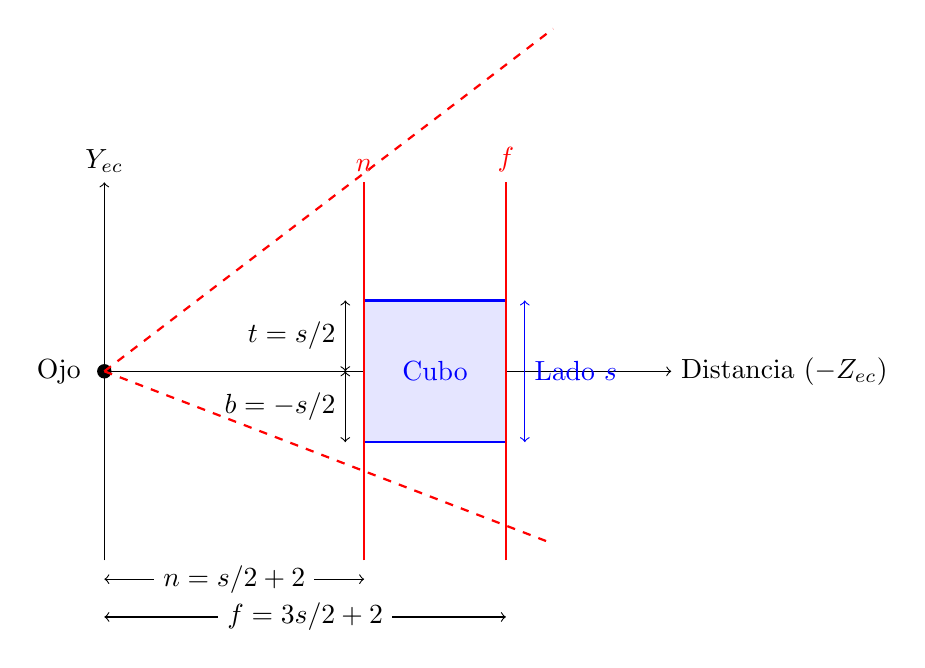
\begin{tikzpicture}[scale=1.2]
        % Definir parámetros visuales
        \def\eye{0}
        \def\s{1.5} % Tamaño visual del lado s
        \def\gap{2} % El ''+2'' del enunciado
        \def\dist{\s + \gap} % Distancia al centro = s + 2
        \def\near{\dist - \s/2} % n
        \def\far{\dist + \s/2}  % f
        \def\halfS{\s/2}
        
        % Eje Z negativo (hacia donde miramos)
        \draw[->] (0,0) -- (6,0) node[right] {Distancia ($-Z_{ec}$)};
        \draw[->] (0,-2) -- (0,2) node[above] {$Y_{ec}$};
        
        % El Ojo
        \filldraw (0,0) circle (2pt) node[left=5pt] {Ojo};
        
        % El Cubo
        \draw[blue, thick, fill=blue!10] (\near, -\halfS) rectangle (\far, \halfS);
        \node[blue] at (\dist, 0) {Cubo};
        \draw[<->, blue] (\far+0.2, -\halfS) -- (\far+0.2, \halfS) node[midway, right] {Lado $s$};
        
        % Planos Near y Far
        \draw[red, thick] (\near, -2) -- (\near, 2) node[above] {$n$};
        \draw[red, thick] (\far, -2) -- (\far, 2) node[above] {$f$};
        
        % Líneas de visión (Frustum)
        % Conectan el ojo con los bordes de la cara delantera (que define el recorte)
        \draw[dashed, thick, red] (0,0) -- (\far+0.5, {(\far+0.5)*\halfS/\near});
        \draw[dashed, thick, red] (0,0) -- (\far+0.5, {-(\far+0.5)*\halfS/\near - 0.7});
        
        % Cotas explicativas
        \draw[<->] (0, -2.2) -- (\near, -2.2) node[midway, fill=white] {$n = s/2 + 2$};
        \draw[<->] (0, -2.6) -- (\far, -2.6) node[midway, fill=white] {$f = 3s/2 + 2$};
        
        % Top y Bottom
        \draw[<->] (\near-0.2, 0) -- (\near-0.2, \halfS) node[midway, left] {$t=s/2$};
        \draw[<->] (\near-0.2, 0) -- (\near-0.2, -\halfS) node[midway, left] {$b=-s/2$};
        
    \end{tikzpicture}
    \end{center}

    \item \textbf{Resultado Final:}
    Los valores calculados únicamente en función de $s$ son:
    \[ n = \frac{s}{2} + 2, \quad f = \frac{3s}{2} + 2 \]
    \[ r = \frac{s}{2}, \quad l = -\frac{s}{2}, \quad t = \frac{s}{2}, \quad b = -\frac{s}{2} \]
\end{enumerate}
\end{solucion}

\begin{ejercicio}
Repetimos el problema 6.7 con los mismos requerimientos y suposiciones, pero ahora la escena está contenida en una esfera de radio $r$ con centro en $c=(c_x, c_y, c_z)$, en lugar de un cubo.

\textbf{Datos y Adaptación del Enunciado:}
\begin{itemize}
    \item Objeto: Esfera de radio $r$.
    \item Centro: $c = (c_x, c_y, c_z)$.
    \item Cámara: Para mantener la equivalencia con el ejercicio anterior (donde la distancia dependía del tamaño del objeto $s$), sustituimos el lado del cubo $s$ por el diámetro de la esfera $2r$.
    \item Posición de la cámara: $o_{ec} = (c_x, c_y, c_z + 2r + 2)$.
    \item Orientación: Mira hacia $c$, vector arriba $(0,1,0)$.
\end{itemize}

\textbf{Requerimientos:}
\begin{itemize}
    \item $n$ y $f$ ajustados al máximo al objeto.
    \item Tamaño aparente máximo sin recortar (la esfera debe entrar completa en la imagen).
    \item Viewport cuadrado (aspect ratio 1).
\end{itemize}
\end{ejercicio}

\begin{solucion}
Procederemos de forma análoga al caso del cubo, utilizando la \textbf{caja englobante} (bounding box) de la esfera para asegurar que esta quede completamente dentro del volumen de vista. Una esfera de radio $r$ cabe perfectamente dentro de un cubo de lado $s = 2r$.

\begin{enumerate}
    \item \textbf{Paso 1: Análisis de Distancias en el Eje Z.}
    
    Transformamos el centro de la esfera a coordenadas de cámara (poniendo la cámara en el origen).
    La distancia $D$ desde el ojo hasta el centro $c$ es la diferencia en la coordenada $Z$:
    \[ D = Z_{ojo} - Z_{centro} = (c_z + 2r + 2) - c_z = 2r + 2 \]
    
    La esfera se extiende una distancia $r$ (el radio) hacia adelante y hacia atrás desde su centro.
    
    \item \textbf{Paso 2: Cálculo de los planos de recorte ($n$ y $f$).}
    
    \begin{itemize}
        \item \textbf{Plano Near ($n$):} Debe situarse justo delante del punto más cercano de la esfera.
        \[ n = D - \text{radio} = (2r + 2) - r = r + 2 \]
        
        \item \textbf{Plano Far ($f$):} Debe situarse justo detrás del punto más lejano de la esfera.
        \[ f = D + \text{radio} = (2r + 2) + r = 3r + 2 \]
    \end{itemize}

    \item \textbf{Paso 3: Cálculo de la ventana de proyección ($l, r, b, t$).}
    
    Para asegurar que la esfera se vea completa y lo más grande posible, ajustaremos el frustum para que englobe el cuadrado frontal de la ''caja imaginaria'' que contiene a la esfera.
    
    Si el plano de proyección está en $n$, la sección de la caja englobante en ese plano tiene una altura y anchura igual al diámetro de la esfera ($2r$). Sin embargo, debido a la perspectiva, si ajustamos la ventana para cubrir el tamaño del objeto en el plano $near$, garantizamos que cualquier parte del objeto detrás de ese plano también será visible (ya que el frustum se ensancha).
    
    La ''cara delantera'' de nuestra caja imaginaria en $z=-n$ tendría un tamaño de $2r \times 2r$. Como la cámara apunta al centro:
    
    \begin{itemize}
        \item Ancho total = $2r \implies$ Del centro a la derecha = $r$.
        \item Alto total = $2r \implies$ Del centro hacia arriba = $r$.
    \end{itemize}
    
    Por tanto:
    \[ r = r \quad (\text{coincide con el radio}) \]
    \[ t = r \]
    \[ l = -r \]
    \[ b = -r \]
    
    \textit{Nota: Al usar $t=r$ en el plano $n$, estamos definiendo un frustum que pasa exactamente por los bordes de la esfera en su punto más cercano. Como la esfera se curva ''hacia adentro'', esto garantiza holgura y que la esfera completa sea visible.}

    \item \textbf{Representación Gráfica:}
    
    El esquema muestra la esfera (azul) y cómo los planos $n$ y $f$ la encierran (rojo).

    \begin{center}
    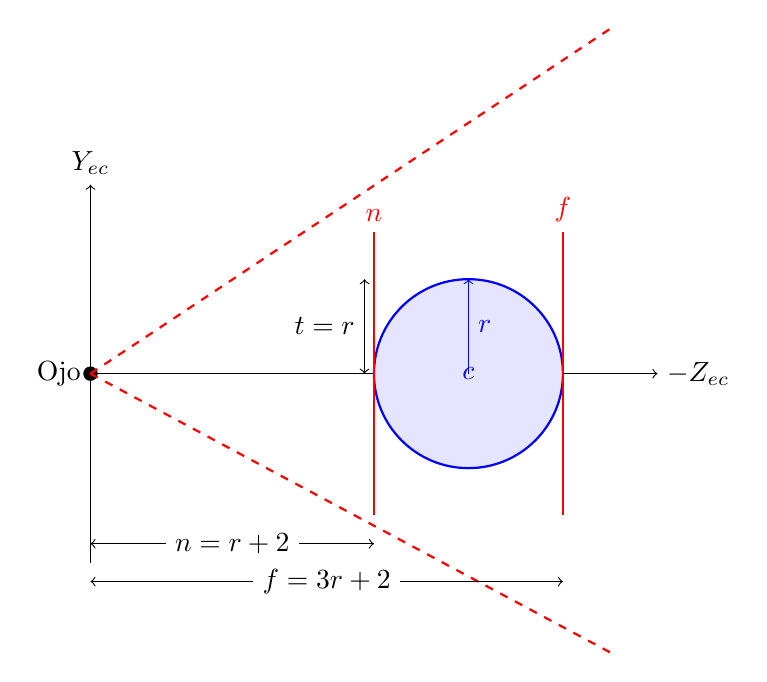
\begin{tikzpicture}[scale=1.2]
        % Definir parámetros
        \def\rad{1.0} % radio r
        \def\gap{2.0} % el +2
        \def\D{2*\rad + \gap} % Distancia D = 2r + 2 = 4
        \def\near{\rad + \gap} % n = r + 2 = 3
        \def\far{3*\rad + \gap} % f = 3r + 2 = 5
        
        % Ejes
        \draw[->] (0,0) -- (6,0) node[right] {$-Z_{ec}$};
        \draw[->] (0,-2) -- (0,2) node[above] {$Y_{ec}$};
        \filldraw (0,0) circle (2pt) node[left] {Ojo};
        
        % Esfera
        \draw[blue, thick, fill=blue!10] (\D, 0) circle (\rad);
        \node[blue] at (\D, 0) {$c$};
        \draw[blue, ->] (\D, 0) -- (\D, \rad) node[midway, right] {$r$};
        
        % Planos Near y Far
        \draw[red, thick] (\near, -1.5) -- (\near, 1.5) node[above] {$n$};
        \draw[red, thick] (\far, -1.5) -- (\far, 1.5) node[above] {$f$};
        
        % Frustum (Líneas de visión pasando por r en n)
        % Nota: t=r en distancia n. Pendiente = r/n.
        \draw[dashed, thick, red] (0,0) -- (\far+0.5, {(\far+0.5)*0.3*\rad/\near});
        \draw[dashed, thick, red] (0,0) -- (\far+0.5, {-(\far+0.5)*0.9*\rad/\near});      
        % Cotas
        \draw[<->] (0, -1.8) -- (\near, -1.8) node[midway, fill=white] {$n = r+2$};
        \draw[<->] (0, -2.2) -- (\far, -2.2) node[midway, fill=white] {$f = 3r+2$};
        
        % Top (t)
        \draw[<->] (\near-0.1, 0) -- (\near-0.1, \rad) node[midway, left] {$t=r$};
        
    \end{tikzpicture}
    \end{center}

    \item \textbf{Resumen de resultados:}
    Los parámetros en función de $r$ son:
    \[ n = r + 2, \quad f = 3r + 2 \]
    \[ r_{param} = r, \quad l = -r, \quad t = r, \quad b = -r \]
    (Donde $r_{param}$ es el parámetro \textit{right} del frustum y $r$ es el radio de la esfera).
\end{enumerate}
\end{solucion}

\begin{ejercicio}
Repetimos el problema 6.7 (visualización de un cubo de lado $s$), con los mismos requerimientos de optimización (tamaño máximo, sin recortes, $n$ y $f$ ajustados), pero con una diferencia importante:
El viewport (la ventana donde se dibuja la imagen) ya no es necesariamente cuadrado. Tiene dimensiones de $w$ píxeles de ancho y $h$ píxeles de alto.

\textbf{Datos conocidos:}
\begin{itemize}
    \item Objeto: Cubo de lado $s$, centrado en $c$.
    \item Cámara: Posición $o_{ec} = (c_x, c_y, c_z + s + 2)$, mirando a $c$.
    \item Viewport: Resolución $w \times h$. Relación de aspecto $aspect = w/h$.
\end{itemize}

\textbf{Objetivo:} Calcular $n, f, l, r, b, t$ para que el cubo llene la pantalla lo máximo posible sin perder la proporción (sin deformarse) y sin recortarse.
\end{ejercicio}

\begin{solucion}
Este problema introduce el concepto de \textbf{Relación de Aspecto (Aspect Ratio)}. Si la ventana de nuestro programa es rectangular, el volumen de vista (frustum) también debe ser rectangular con la misma proporción, o de lo contrario el cubo se verá estirado o aplastado.

\begin{enumerate}
    \item \textbf{Paso 1: Planos de profundidad ($n$ y $f$).}
    
    La forma del viewport (rectangular o cuadrada) no afecta a la profundidad. La distancia de la cámara al objeto sigue siendo la misma que en el problema 6.7.
    
    Distancia al centro: $D = s + 2$.
    
    Los planos $n$ y $f$ dependen solo de la coordenada Z del cubo:
    \[ n = \frac{s}{2} + 2 \]
    \[ f = \frac{3s}{2} + 2 \]
    
    (Estos valores son idénticos al problema 6.7).

    \item \textbf{Paso 2: Relación de Aspecto.}
    
    Definimos la relación de aspecto del viewport como:
    \[ a = \frac{\text{ancho}}{\text{alto}} = \frac{w}{h} \]
    
    Para evitar deformaciones, las dimensiones físicas de la ventana de proyección ($r-l$ y $t-b$) deben mantener esta misma proporción:
    \[ \frac{r - l}{t - b} = \frac{2r}{2t} = \frac{r}{t} = a \implies r = t \cdot a \]
    (Asumiendo simetría $r = -l$ y $t = -b$).

    \item \textbf{Paso 3: Cálculo de la ventana ($l, r, b, t$).}
    
    La cara del cubo que debemos encuadrar es un \textbf{cuadrado de lado $s$}.
    Tenemos que meter ese cuadrado de tamaño $s \times s$ dentro de un rectángulo de proporción $w \times h$.
    
    Debemos distinguir dos casos posibles para garantizar que el cubo entre entero (''tamaño aparente mayor posible'' significa ajustar a la dimensión más restrictiva).

    \textbf{CASO A: Viewport Apaisado o ''Landscape'' ($w \ge h$)}
    \begin{itemize}
        \item La ventana es más ancha que alta.
        \item Si ajustamos el ancho de la ventana al ancho del cubo ($2r = s$), la altura de la ventana ($2t$) sería proporcionalmente menor a $s$, y cortaríamos el cubo por arriba y abajo.
        \item \textbf{Solución:} El factor limitante es la \textbf{altura}. Debemos igualar la altura de la ventana a la altura del cubo.
        \[ t = \frac{s}{2}, \quad b = -\frac{s}{2} \]
        \item El ancho se ajusta automáticamente para mantener la proporción (será mayor que $s$, dejando espacio libre a los lados):
        \[ r = t \cdot \frac{w}{h} = \frac{s}{2} \cdot \frac{w}{h} \]
        \[ l = -r = -\frac{s}{2} \cdot \frac{w}{h} \]
    \end{itemize}

    \textbf{CASO B: Viewport Vertical o ''Portrait'' ($w < h$)}
    \begin{itemize}
        \item La ventana es más alta que ancha.
        \item Si ajustamos la altura de la ventana a la altura del cubo ($2t = s$), el ancho ($2r$) sería menor que $s$, y cortaríamos el cubo por los lados.
        \item \textbf{Solución:} El factor limitante es el \textbf{ancho}. Debemos igualar el ancho de la ventana al ancho del cubo.
        \[ r = \frac{s}{2}, \quad l = -\frac{s}{2} \]
        \item La altura se ajusta automáticamente (será mayor que $s$, dejando espacio libre arriba y abajo):
        \[ t = \frac{r}{a} = r \cdot \frac{h}{w} = \frac{s}{2} \cdot \frac{h}{w} \]
        \[ b = -t = -\frac{s}{2} \cdot \frac{h}{w} \]
    \end{itemize}

    \item \textbf{Resumen Gráfico de los Casos:}

    \begin{center}
    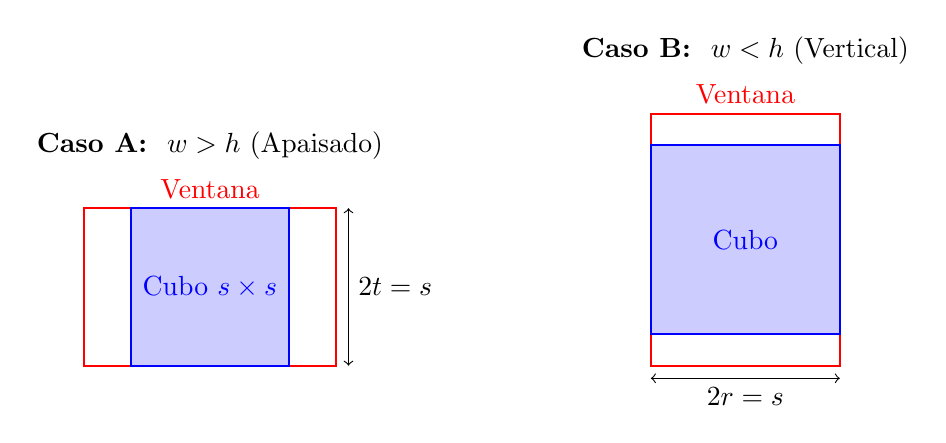
\begin{tikzpicture}[scale=0.8]
        % Caso A: Landscape
        \node at (2, 3.5) {\textbf{Caso A: } $w > h$ (Apaisado)};
        % Viewport (Rectángulo rojo)
        \draw[red, thick] (0,0) rectangle (4, 2.5);
        \node[red, above] at (2, 2.5) {Ventana};
        % Cubo (Cuadrado azul)
        % Ajustado en altura
        \draw[blue, thick, fill=blue!20] (0.75, 0) rectangle (3.25, 2.5);
        \node[blue] at (2, 1.25) {Cubo $s \times s$};
        \draw[<->] (4.2, 0) -- (4.2, 2.5) node[midway, right] {$2t = s$};

        % Más separación entre los dos casos
        \begin{scope}[xshift=9cm] % antes era 6cm, ahora 9cm para más separación
            \node at (1.5, 5) {\textbf{Caso B: } $w < h$ (Vertical)};
            % Viewport (Rectángulo rojo)
            \draw[red, thick] (0,0) rectangle (3, 4);
            \node[red, above] at (1.5, 4) {Ventana};
            % Cubo (Cuadrado azul)
            % Ajustado en anchura
            \draw[blue, thick, fill=blue!20] (0, 0.5) rectangle (3, 3.5);
            \node[blue] at (1.5, 2) {Cubo};
            \draw[<->] (0, -0.2) -- (3, -0.2) node[midway, below] {$2r = s$};
        \end{scope}
    \end{tikzpicture}
    \end{center}

    \item \textbf{Resultado General Unificado:}
    Podemos expresar la solución usando la función máximo para cubrir ambos casos:
    \[ n = \frac{s}{2} + 2, \quad f = \frac{3s}{2} + 2 \]
    \[ r = \frac{s}{2} \cdot \max\left(1, \frac{w}{h}\right), \quad t = \frac{s}{2} \cdot \max\left(1, \frac{h}{w}\right) \]
    \[ l = -r, \quad b = -t \]
\end{enumerate}
\end{solucion}

\begin{ejercicio} \textbf{Alta complejidad.}
Posicionamiento de cámara dado un FOV ($\beta$).

Repetimos el problema 6.7 (cubo de lado $s$ centrado en $c$), manteniendo los requerimientos de optimización (viewport cuadrado, sin recortes, $n$ máximo, $f$ mínimo).

\textbf{Nueva condición:}
En lugar de darnos la posición de la cámara, se nos da el ángulo de apertura vertical (Field of View) $\beta$.
Debemos calcular:
\begin{enumerate}
    \item La coordenada Z de la posición del observador ($o_{ec}$), sabiendo que $o_x = c_x$ y $o_y = c_y$.
    \item Los parámetros de la proyección $l, r, t, b, n, f$ en función de $\beta, s$ y $c$.
\end{enumerate}
\end{ejercicio}

\begin{solucion}
Este problema es ''inverso'' al anterior en cierto sentido. Antes fijábamos la distancia y calculábamos qué apertura necesitábamos (implícitamente). Ahora, fijamos la apertura (el ángulo de la lente) y tenemos que calcular a qué distancia ponernos para que el cubo llene la pantalla perfectamente.

\begin{enumerate}
    \item \textbf{Paso 1: Entender la geometría del FOV ($\beta$).}
    
    El ángulo $\beta$ es la apertura total vertical. La mitad de ese ángulo es $\beta/2$.
    En un triángulo rectángulo formado por la línea de visión, el plano de proyección y el borde superior del frustum:
    \[ \tan(\beta/2) = \frac{\text{altura del marco}}{\text{distancia al marco}} = \frac{t}{n} \]
    
    Queremos que el cubo llene la pantalla. Esto ocurre cuando el ''marco'' de visión en el plano más cercano ($n$) coincide exactamente con la cara delantera del cubo.
    
    La cara delantera del cubo tiene altura $s$. Por tanto, desde el centro hacia arriba mide $s/2$.
    Esto fija nuestro valor de $t$:
    \[ t = \frac{s}{2} \]

    \item \textbf{Paso 2: Calcular la distancia al plano Near ($n$).}
    
    Sustituimos $t$ en la ecuación del FOV y despejamos $n$:
    \[ \tan(\beta/2) = \frac{s/2}{n} \]
    \[ n = \frac{s/2}{\tan(\beta/2)} = \frac{s}{2} \cdot \cot(\beta/2) \]
    
    Ahora ya sabemos cuánto espacio debe haber entre el ojo y la cara delantera del cubo ($n$).

    \item \textbf{Paso 3: Calcular la posición de la cámara ($o_z$).}
    
    Sabemos dónde está el cubo en el mundo (en $c_z$).
    \begin{itemize}
        \item El centro del cubo está en $c_z$.
        \item La cara delantera está en $c_z + s/2$ (hacia nosotros).
        \item El ojo está una distancia $n$ más allá de la cara delantera.
    \end{itemize}
    
    \[ o_z = \text{Posición cara delantera} + n \]
    \[ o_z = (c_z + \frac{s}{2}) + n \]
    
    Sustituyendo el valor de $n$ calculado antes:
    \[ o_z = c_z + \frac{s}{2} + \frac{s}{2}\cot(\beta/2) = c_z + \frac{s}{2} \left( 1 + \cot(\frac{\beta}{2}) \right) \]
    
    Por tanto, la posición del observador es:
    \[ o_{ec} = \left( c_x, c_y, c_z + \frac{s}{2} \left( 1 + \cot(\frac{\beta}{2}) \right) \right) \]

    \item \textbf{Paso 4: Calcular el resto de parámetros ($f, l, r, b$).}
    
    \begin{itemize}
        \item \textbf{$f$ (Far):} Es la distancia desde el ojo hasta la cara trasera. La cara trasera está a una distancia $s$ (la profundidad del cubo) más lejos que la cara delantera ($n$).
        \[ f = n + s \]
        \[ f = \frac{s}{2}\cot(\beta/2) + s \]
        
        \item \textbf{$t, b, l, r$:} Como el viewport es cuadrado (según enunciado 6.7) y queremos ajustar a la cara delantera ($s \times s$):
        \[ t = \frac{s}{2} \]
        \[ b = -\frac{s}{2} \]
        \[ r = \frac{s}{2} \]
        \[ l = -\frac{s}{2} \]
    \end{itemize}

    \item \textbf{Esquema Gráfico:}
    
    El diagrama muestra cómo el ángulo $\beta$ determina la distancia $n$ para que el frustum coincida con la altura $s/2$.

    \begin{center}
    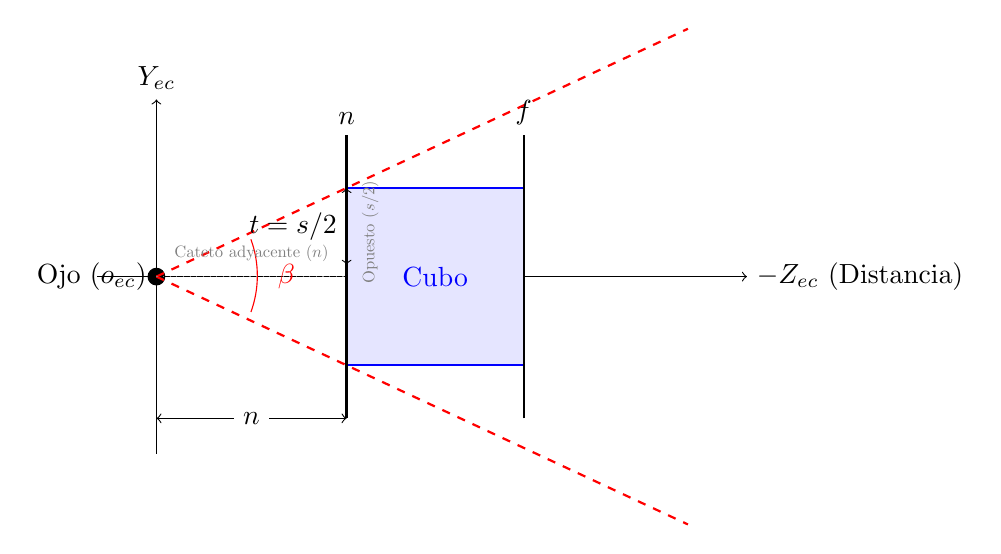
\begin{tikzpicture}[scale=1.5]
        % Parámetros
        \def\angle{25} % beta/2 aprox
        \def\h{0.75}   % s/2
        \def\n{1.61}   % n calculado manualmente para evitar problemas con tan()
        \def\s{1.5}    % s = 2*h
        \def\front{\n}
        \def\back{\n + \s}
        \def\centerZ{\n + 0.5*\s}
        
        % Eje Z
        \draw[->] (-0.5,0) -- (5,0) node[right] {$-Z_{ec}$ (Distancia)};
        \draw[->] (0,-1.5) -- (0,1.5) node[above] {$Y_{ec}$};
        \filldraw (0,0) circle (2pt) node[left] {Ojo ($o_{ec}$)};
        
        % Cono de visión (FOV)
        \draw[red, thick, dashed] (0,0) -- (4.5, {4.5*tan(\angle)});
        \draw[red, thick, dashed] (0,0) -- (4.5, {-4.5*tan(\angle)});
        
        % Arco beta
        \draw[red] (0.8, -0.3) arc (-20:20:0.9);
        \node[red] at (1.1, 0) {$\beta$};
        
        % Cubo
        \draw[blue, thick, fill=blue!10] (\front, -\h) rectangle (\back, \h);
        \node[blue] at (\centerZ, 0) {Cubo};
        
        % Planos n y f
        \draw[thick] (\front, -1.2) -- (\front, 1.2) node[above] {$n$};
        \draw[thick] (\back, -1.2) -- (\back, 1.2) node[above] {$f$};
        
        % Cotas y relaciones
        \draw[<->] (\front, 0.1) -- (\front, \h) node[midway, left] {$t=s/2$};
        \draw[<->] (0, -1.2) -- (\front, -1.2) node[midway, fill=white] {$n$};
        
        % Triángulo explicativo
        \draw[gray, dotted] (0,0) -- (\front, 0);
        \node[gray, scale=0.6] at ({0.5*\front}, 0.2) {Cateto adyacente ($n$)};
        \node[gray, scale=0.6, rotate=90] at ({\front+0.2}, {0.5*\h}) {Opuesto ($s/2$)};
    \end{tikzpicture}
    \end{center}

    \item \textbf{Resumen de Fórmulas:}
    \[ o_z = c_z + \frac{s}{2} \left( 1 + \cot\frac{\beta}{2} \right) \]
    \[ n = \frac{s}{2} \cot\frac{\beta}{2} \]
    \[ f = n + s \]
    \[ r = t = \frac{s}{2}, \quad l = b = -\frac{s}{2} \]
\end{enumerate}
\end{solucion}